
%
% ---- Chapter layout ----
%
% 1) Introduction - 
% 2) 
% ------------------------



\chapter{Biogenic Isoprene emissions in Australia} % Chapter title
\label{BioIsop}
  
%----------------------------------------------------------------------------------------
% Section 1 -- INTRO 
%----------------------------------------------------------------------------------------
\section{Introduction}  
\label{BioIsop:intro}  
  
  
  
  % isoprene and Australia
  Biogenic volatile organic compounds (BVOC) affect the oxidative capacity of the atmosphere and are largely driven by what type of vegetation is in the area \parencite{Kefauver2014}.
  In the troposphere, BVOC emissions affect hydroxyl radical (OH) cycling, ozone (O$_3$) and secondary organic aerosol (SOA) production, and methane lifetime.
  Australian forests are strong emitters of isoprene, the primary BVOC emitted globally \parencite{Guenther2006,Messina2016}. % and monoterpenes.
  Poor measurement coverage of isoprene, isoprene products, and isoprene emissions within Australia means that emissions are poorly understood.
  The lack of measurements makes it difficult to estimate the subsequent atmospheric processes. 
  Isoprene (C$_5$H$_8$) is relatively difficult to measure due to its high reactivity and short lifetime.
  
  Emission models used to derive estimates of isoprene fluxes are based on understanding the emissions from different plant species (phenotypes) in varying conditions.
  \textcite{Guenther2012} estimated global biogenic isoprene emissions at roughly 535\tgpyr, while \textcite{Sindelarova2014} estimated around 411\tgpyr.
  %Guenther used MEGAN, \textcite{Sindelarova2014} estimated around 594\tgpyr using MEGAN with MACC, showing isoprene as 69.2\% of the total BVOC emissions, with monoterpenes at 10.9\tgpyr (10.9\%).
  Reactions following emissions are complex, and are sensitive to other trace gases in the ambient atmosphere.
  Uncertainties in several important products such as ozone and SOA are increased due to both isoprene measurement difficulties and its complicated subsequent chemical mechanisms.
  Isoprene emissions may be overestimated in Australia since they are based on measurements taken from a few young trees \parencite{Winters2009} that may emit more than older trees \parencite{Emerson2016}.
  The sample of trees include 4 types of Eucalyptus, which are not representative of the hundreds of species that make up Australian forests, and how these species depend on biological and meteorological stresses is unclear \parencite{Winters2009, FortemsCheiney2012}.
  Emissions estimates are often used as boundary conditions for atmospheric chemistry models and improving these estimates for Australia is one goal of this thesis.
  %without an expensive measurement campaign over the large data sparse continent of Australia.
  %%BVOC emissions are rising globally, and improving estimates for Australia is a priority since they affect such important processes in the atmosphere.
  %\textcite{Kefauver2014} reviews remote sensing of BVOC emissions, examining the last 20 years of data and analysis of the satellite products.
  
  
  In this chapter I describe and implement a \textit{top down} technique using satellite measurements of HCHO to calculate surface isoprene emissions.
  HCHO is a dominant product of most BVOCs, including isoprene, and is measured by satellites via remote sensing.
  In situ isoprene concentration measurements are costly and sparse within Australia, while satellite HCHO data are plentiful and freely available, making this technique very attractive.
  Top down techniques have informed isoprene emission inventories in North America \parencite{Abbot2003,Palmer2003,Palmer2006,Millet2006,Millet2008}, South America \parencite{Barkley2013}, Europe \parencite{Dufour2009,Curci2010}, Africa \parencite{Marais2012}, Asia \parencite{Fu2007,Stavrakou2014}, India \parencite{Surl2018}, and even globally \parencite{Shim2005,FortemsCheiney2012,Bauwens2016}.
  In this thesis I apply the technique solely focusing on Australia for the first time.
  % Too specific
  %In this thesis the OMHCHO dataset from the OMI instrument (see Section \ref{Model:omhcho}) is used as the basis for HCHO amounts.
  
  \subsection{Aims}
    \label{BioIsop:intro:aims}
    
    %% AIMs paragraph
    Recent work suggests that modelled emissions may be overestimated in Australia \parencite{Emmerson2016}.
    %, while emissions of monoterpenes (C$_{10}$H$_{16}$, two units of isoprene) appear to be underestimated . 
    %This could lead to the unique scenario of neither emission type dominating VOC chemistry over the forests.
    This work tries to improve the understanding of isoprene emissions over the whole of Australia, clarifying the spatial distribution of bias and how these biases impact modelled chemistry.
    I estimate isoprene emissions in Australia using a top-down technique based on OMI HCHO measurements and GEOS-Chem modelled yields.
    This a posteriori top-down estimate is then evaluated against sparse available ground-based measurements.
    The GEOS-Chem model is modified to run with the a posteriori isoprene emissions to determine potential impact on modelled chemistry.
    Goodness of fit between in situ, satellite, and modelled HCHO is determined before and after scaling emissions estimates.
    
    
    In this chapter I outline why current isoprene emissions estimates are inadequate and how they can be improved.
    I discuss literature that shows how the estimates may be too high, and describe how emissions may be calculated using satellite datasets.
    Section \ref{BioIsop:method} lays out how new isoprene emissions are estimated, with results examined in Section \ref{BioIsop:results}. 
    Updated satellite HCHO columns (Chapter \ref{Model}) are compared to available measurements in Section \ref{BioIsop:results:measurements}.
    %(SPS1, SPS2, MUMBA, Wollongong FTIR)
    Uncertainties for each step along the way are quantified in Section \ref{BioIsop:uncertainty}.
    In Section \ref{BioIsop:conclusions} I examine how these changes in emissions would affect ozone concentrations in Australia, along with some other chemical processes.
    
    
  \subsection{Existing emissions estimates}
    

    % Overestimates from models
    The Model of Emissions of Gases and Aerosols from Nature (MEGAN) is one of the most widely used sources for biogenic isoprene.
    Along with other models that rely on measured plant emission rates, it is poorly calibrated for Australian conditions.
    Emissions of isoprene (C$_5$H$_8$) appear to be overestimated in within Australia \parencite{Sindelarova2014,Stavrakou2014,Emmerson2016}.
    Although the lack of measurements of isoprene emission rates in Australia makes this overestimation difficult to characterise.
    \textcite{Stavrakou2015} saw isoprene emissions overestimated by a factor of 2-3 in January.
    \textcite{Emmerson2016} suggest isoprene emissions are estimated 2-6 times too high compared against available measurements of isoprene concentrations.
    They also show that no blanket increase or decrease in emission factors is appropriate for the entire southeast of Australia.
    They compared modelled data to campaign measurements from multiple sites over different seasons and found that scaling emissions did not universally improve model outputs.
    % Not relevant
    %Additionally, emissions of monoterpenes (C$_{10}$H$_{16}$, two units of isoprene) appear to be underestimated \parencite{Emmerson2016}.
    %This could lead to the unique scenario of neither emission type dominating VOC chemistry over the forests.
    

    Recently \textcite{Bauwens2016} estimated isoprene emissions with a top-down technique using the IMAGESv2 global CTM.
    They calculated emissions that create the closest match between model and satellite vertical columns, and compared these a posteriori data with their a priori (model data) and independent data sets.
    %They examine global emissions seen by three models and a top-down inversion. % this is just what they do, not results etc...
    For Australia they found emissions ranging from 26-94\tgcpyr, with MEGAN a priori emissions of 38\tgcpyr and a posteriori emissions of 36\tgcpyr, although the 94\tgcpyr estimate was also based on MEGAN.
    In this thesis I focus on the analysis of a top-down emissions estimate compared against MEGAN, along with how changed emissions affect modelled ozone levels.
  
  \subsection{Top-down isoprene emissions estimates}
    \label{BioIsop:intro:top_down_estimates}
    
    % Brief isoprene to hcho description
    In the remote troposphere HCHO production is dominated by methane oxidation, while in the continental boundary layer production is largely due to non-methane VOCs (NMVOCs) \parencite{Abbot2003, Kefauver2014}.
    This leads to a causal relationship between enhanced HCHO concentrations and NMVOC emissions at low ($<1$~km) altitudes.
    NMVOCs are generally short lived ($<1$~hr), and the most prominent of these is isoprene.
    Isoprene is emitted and enters the atmosphere in the gas phase, where it begins a complex series of reactions.
    HCHO is produced with high yield in many reactions beginning with isoprene oxidation, discussed in more detail in Section \ref{LR:VOCs:IsopCascade}, and has a lifetime of a few hours \parencite{Kefauver2014}.
    
    % Lead in to satellite inversion
    Top-down estimates determine emissions of a particular species through careful analysis of the measurable products of that species.
    This generally takes advantage of longer-lived products that may reach an equilibrium in the atmosphere.
    For isoprene this is done through examination of atmospheric HCHO enhancement, which is a major product of isoprene oxidation that takes place after emission.
    %Even anthropogenic HCHO source estimates, which are accurate at the global scale, can be improved using satellite data to improve regional estimates by up to 25-40\% \parencite{Stavrakou2015}. 
    %Their study used the RETRO 2000 database for anthropogenic emission a prioris except for Asia in 2008 where REASv2 was used. 
    Since 1997, when GOME measurements were first used to measure HCHO over Asia, satellites have been used to provided a total column measurement of HCHO, providing isoprene emissions estimation by top-down methods \parencite{Thomas1998,Palmer2001,Bauwens2016}.
    Using satellite information to improve estimates of biogenic emissions has been highlighted as a valuable use of satellite derived datasets \parencite{Streets2013}.
    Here NASA's OMHCHO product based on measurements from the OMI instrument onboard the Aura satellite (see Section \ref{Model:omhcho}) is the basis for a top down biogenic isoprene emission estimate over Australia.
    
    There are two top-down isoprene emission estimation techniques, Bayesian and linear, which are discussed briefly here.
    Both the linear and Bayesian techniques assume that modelled chemistry is accurate and only try to correct precursor emissions.
    This is an additional source of uncertainty given existing uncertainties in chemical mechanisms.
    
    
    %    Top-down emission estimation is an in-depth process, and a couple of examples are provided here.
    %    \textcite{Marais2014} compare OMI based isoprene emission estimates against relaxed eddy accumulation measurements from African field campaigns in order to improve MEGAN emission factors in the region.
    %    \textcite{Dufour2009} use HCHO from SCIAMACHY, and examine Europe using CHIMERE as the chemical model, showing that satellite measurements can reduce source emission uncertainty by a factor of two, where emissions are relatively large.
    %    There are two main methods of estimating isoprene emissions using satellite measurements of child products, here I describe them and briefly compare the pros and cons of each.
    %    
    
    
    \subsubsection{Bayesian inversion}
    
      % Top down emissions estimation methods:
      Bayesian inversion optimises model parameters in order to minimise the difference between model output and an (ideally) independent dataset such as satellite measurements.
      Emissions of isoprene (and other precursors to HCHO) will form part of the set of model parameters that are adjusted to make the model HCHO output most closely match satellite measurements.
      These inversions can be set up to account for effects from transport and allow source attribution \parencite[e.g.][]{Curci2010,FortemsCheiney2012}.
      
      In general; a model (the forward model) is used to determine the relationship between HCHO ($y$) and the state variable \emph{x}, which represents isoprene emissions (and other variable parameters of interest):
      \begin{equation}
        \label{BioIsop:intro:top_down_estimates:eqn_bayesian}
        y=\mathbf{Kx} + b + \epsilon
      \end{equation}
      where $\epsilon$ are the (assumed) independent errors in measurements.
      \emph{K} is the Jacobian matrix determined from the forward model representing the sensitivity of $y$ to the state variable \emph{x}.
      Essentially the \emph{K} matrix is the modelled estimation of how $y$ responds to each of the driving parameters represented by elements of \emph{x}
      This \emph{K} matrix is used in conjunction with error covariance in \emph{x} to determine the most likely solution to \emph{x}, given what is known about $y$. % ($\hat{x}$).
      
      % Some examples:
      This method was used by \textcite{Shim2005} to optimise isoprene emissions in areas with high HCHO concentrations. 
      % improve comparison against GOME HCHO observations.
      They showed model underestimation of isoprene emissions by 14-46\%, which when corrected reduced bias between GOME HCHO measurements and GEOS-Chem model output by 3-25\%.
      More recently \textcite{Kaiser2018} showed a 40\% bias in MEGAN isoprene emissions over the southeast US using a Bayesian inversion based on OMI HCHO.
      %An example showing how regional anthropogenic VOC emissions estimates can be improved using OMI HCHO observations and the CHIMERE CTM can be found in \textcite{Curci2010}.
      %The Bayesian inversion is also used in \textcite{Curci2010}, where a regional CTM (CHIMERE) simulates HCHO (this is the forward model), which is compared against OMI observed HCHO and shown to be regionally biased.
      %The CHIMERE model is used to derive yields of HCHO from the various local VOCs and these are then used in estimating local emissions.
      %The model is run initially with emissions of BVOCs and reactive anthropogenic VOCs turned off in order to work out the background ($b$) values of these compounds.
      %They use CHIMERE as the forward model to determine the relationship between HCHO and \emph{x}, which in this case is isoprene and reactive anthropogenic VOCs, then they calculate the most likely values for \emph{x} given known measured HCHO and modelled \emph{K}.
      
      An advantage (over the linear method described below) of the Bayesian method is that it can account for pyrogenic and anthropogenic emissions, as these form part of the state variable $x$.
      However, biases may still arise due to errors in modelled emission estimation \parencite{Curci2010}.
      More limiting is the fact that the Bayesian method is computationally expensive due to the requirement that model runs take place using many permutations of changed input parameters.
      In this work I do not use the Bayesian method due to the computational costs surpassing the resources available.
      
    \subsubsection{Linear inversion}
      \label{BioIsop:intro:top_down_linear}
      
      % Technique summary
      The linear technique is the less complicated of the two, and is performed in this thesis.
      Vertical columns of HCHO from satellite and modelled yield from isoprene allow the inference of local (grid space) isoprene emissions \parencite{Palmer2003, Millet2006,Marais2012,Bauwens2016}.
      In Australia the effective molar HCHO yield from isoprene has not been extensively studied, while in other continents this value varies from 1-3 depending on local NO$_x$ concentrations \parencite[e.g.][]{Palmer2006, Millet2006, Bauwens2016, Surl2018}.
      %This yield is derived from both HCHO and isoprene, such as was used by \textcite{Millet2006} who produced a molar HCHO yield of 2.3 in north eastern USA.
      The primary assumption of the linear inversion technique is that HCHO and its precursors (primarily isoprene) are in a linear steady state relationship.
      This allows one to link isoprene emissions to HCHO measurements using production and loss rates.
      Essentially a linear relationship between total column HCHO ($\Omega$) enhancement above a background level ($\Omega_0$) and isoprene emissions ($E_{isop}$) is determined:
      \begin{equation*}
        \Omega = S \times E_{isop} + \Omega_0
      \end{equation*}
      This uses modelled vertical columns and emissions to estimate the slope ($S$).
      Then this modelled $S$ is applied to satellite measurements of $\Omega$ ($\Omega_{sat}$ and $\Omega_{sat,0}$ to determine $\hat{E_{isop}}$:
      \begin{equation*}
        \hat{E_{isop}} = \frac{\Omega_{sat} - \Omega_{sat,0}}{S}
      \end{equation*}
      This is described further in Section \ref{BioIsop:method}, with an outline in Section \ref{BioIsop:method:outline}.
      
      % how palmer did it
      The calculation requires reaction rates and yields from isoprene to HCHO, which can be determined most readily using chemical modelling.
      The method for calculating isoprene emissions from HCHO is laid out in \textcite{Palmer2003}, taking into account the expected lifetime and reaction rates of the precursor VOCs and HCHO.
      In their work, isoprene emissions fluxes over the US were derived using the Global Ozone Monitoring Experiment (GOME) satellite instrument.
      The method has since been applied to many regions using OMI, GOME, GOME-2, and SCIAMACHY satellite data \parencite[e.g.][]{Abbot2003, Barkley2013, Stavrakou2014, Surl2018}.
      % Abbot2003, Millet2006 - GOME
      % Stavrakou2014 - GOME2
      % Marais2012, Surl2018 - OMI
      % Dufour2009, Barkley2013 - SCIAMACHY
      %Palmer's method improved biogenic isoprene emissions estimates (compared with in situ measurements) over two available inventories: the U.S. EPA Biogenic Emissions Inventory System and the Global Emissions Inventory Activity. %(BEIS2)(GEIA).
      %\parencite{Abbot2003,Palmer2003,Palmer2006,Millet2006,Millet2008}, South America \parencite{Barkley2013}, Europe \parencite{Dufour2009,Curci2010}, Africa \parencite{Marais2012}, Asia \parencite{Fu2007,Stavrakou2014}, India \parencite{Surl2018}, and even globally \parencite{Shim2005,FortemsCheiney2012,Bauwens2016}.
      In this thesis I apply the technique solely focusing on Australia for the first time.
      % Too specific
      %In this thesis the OMHCHO dataset from the OMI instrument (see Section \ref{Model:omhcho}) is used as the basis for HCHO amounts.
      
      
      
      % Pros and cons:
      The linear inversion assumes fast HCHO yield from isoprene and no precursor transport, which is unrealistic in certain scenarios; e.g. high wind speeds can transport precursors, or low NO$_x$ concentrations can slow HCHO production \parencite{Palmer2006,Surl2018}.
      Filtering out data that do not match assumptions is required but can limit the utility of this technique, and leads to some dependence on environmental factors.
      %As we are estimating biogenic emissions of isoprene, we must filter out areas where HCHO enhancements arise due to anthropogenic or pyrogenic sources.
      Uncertainties in the technique are discussed in more detail in Section \ref{BioIsop:uncertainty:eomi}.
      Nonetheless, a major benefit is that the simple nature of the inversion requires very little computational power after acquiring satellite and model datasets, even over large amounts of gridded data.
      This allows an inversion using more than 8 years of satellite and model data, capturing inter-annual variability over all of Australia.
      With the computational resources available this would not have been possible using the Bayesian inversion.

\section{Methods}
  \label{BioIsop:method}
  
  
  % First isoprene inversion work
  I broadly follow the method of \textcite{Palmer2001} to create a biogenic isoprene emissions estimate over Australia.
  A relationship is modelled between biogenic-only midday tropospheric columns of HCHO and GEOS-Chem midday biogenic isoprene emission rates, and then this relationship is applied to satellite measured HCHO total columns to derive a new isoprene emissions estimate.
  Daily modelled values averaged between 13:00-14:00~LT are used to match the overpass time of the Aura satellite.
  Then the slope is calculated using the reduced major axis (RMA) regression between the a priori isoprene emissions (those from GEOS-Chem, $\apri$) and tropospheric HCHO columns in each model grid box each month.
  There is very little HCHO above the tropopause, so differences between total and tropospheric column are negligible.
  In this work I refer to both total and tropospheric column HCHO using $\Omega$.
  
  
  \subsection{Outline}
    \label{BioIsop:method:outline}
    % Method Briefly outlined here
    This section provides an overview of the steps involved in creating a top-down emissions estimate. %, from reading satellite data and model output to the creation of isoprene emissions estimates.
    This process is summarised in Figure \ref{BioIsop:method:fig_Flow_Making_Isop}.
    \begin{enumerate}
      \item 
        Corrected vertical columns ($\Oomi$; saved in the OMHCHORP dataset) are calculated (see Section \ref{Model:omiRecalc}) using level two OMI HCHO satellite data (see Section \ref{Model:omhcho}), along with GEOS-Chem model runs (see Section \ref{Model:GC:simulations}).
        Satellite columns are binned into both \highhr and \lowhr horizontal resolutions.
        In this step model background values (columns over the remote pacific) are used to correct the vertical columns, which is explained in Section \ref{Model:omiRecalc:RSC}.
      \item 
        Level three satellite data are used to make anthropogenic, fire, and smoke influence masks (see Section \ref{Model:filter}).
        These are applied to remove $\Oomi$ that may be influenced by pyrogenic or anthropogenic sources. 
      % Mini list for masking taken from here
      \item
        %Modelled slope ($S$) calculations depend on several assumptions that are not always valid.
        A mask is created showing where the HCHO production is not dominated by local isoprene emissions. 
        This is determined by calculating smearing over Australia using two model runs with differing isoprene emissions.
        The smearing value is determined as $\hat{S}=\Delta \Ogc/ \Delta \apost$: the ratio of the differences between model runs of HCHO columns and isoprene emissions.
        The acceptable range for $\hat{S}$ over Australia is determined as 800 - 4600~s.
        A full description of the creation of this smearing filter is given in Section \ref{BioIsop:method:smearing}.
      \item 
        GEOS-Chem modelled biogenic emissions of isoprene ($\apri$) along with biogenic columns of HCHO ($\Ogc$), both averaged over \lowhr ~horizontally and 13:00-14:00~LT temporally, are used to calculate a reduced major axis linear regression slope ($\Ogc=S \times \apri + \Omega_{GC,0}$).
        Calculation of this modelled slope is explained in Section \ref{BioIsop:method:slope}.
      %\item For each of the corrected vertical columns (VCC$_{OMI}$, VCC$_{GC}$, and VCC$_{PP}$; see Section \ref{Model:omiRecalc}), a top down estimate of biogenic isoprene emissions (E$_{new}$; atoms C cm$^{-2}$ s$^{-1}$) is calculated
      \item 
        Satellite HCHO $\Oomi$ and $S$ then form the basis for top-down estimate of biogenic isoprene emissions ($\apost$~atoms C cm$^{-2}$ s$^{-1}$).
        This product is our a posteriori, and calculation details are given in Section \ref{BioIsop:method:calculation}.
      \item 
        A posteriori top-down emissions $\apost$ are compared against a priori emissions, and analysed in conjunction with independent observations from in-situ measurement (MUMBA, and SPS).
        %, and one set of airplane measurements (HIPPO)).
        Results are examined in Section \ref{BioIsop:results}.
      \item 
        GEOS-Chem is run using the a posteriori emissions (see Section \ref{BioIsop:method:scaled}), and HCHO, O$_3$, isoprene, and NO$_x$ outputs are compared to campaign and satellite measurements where possible (Section TODO).
    \end{enumerate}
    
    
    \mypic{Figures/Flow_Making_Isop.png}{%
      Top-down isoprene emissions estimate formation using OMHCHORP and biogenic GEOS-Chem outputs.
      }{\label{BioIsop:method:fig_Flow_Making_Isop}}
  

  \subsection{Masks and reprocessed satellite HCHO}
    
    Satellite data pixels are read from OMHCHO, the level 2 OMI HCHO dataset, AMFs are recalculated, and then pixels are gridded daily into \highhr ~horizontal bins. 
    This forms the intermediate product OMHCHORP, which is fully described in Section \ref{Model:omiRecalc:outline}.
    %In total a month of these data are read in at a time %(to allow parallelism and reduce RAM usage)
    %and then used in subsequent steps to calculate the isoprene emissions.
    This dataset includes gridded satellite HCHO columns ($\Oomi$), along with pixel counts (how many satellite datapoints were used for each grid box) to allow averaging, re-binning, and uncertainty analysis.
    In this thesis I use the OMI product as it has better temporal coverage and increased pixel counts over Australia when compared to GOME or GOME-2 (on board the ERS-2 and METOP-A satellites respectively).
    
    In order to determine biogenic HCHO enhancements from $\Oomi$, we require filters for non-biogenic sources.
    These masks are described in Section \ref{Model:filter}, and a brief recap is provided here.
    While one source of HCHO production is methane oxidation, the linear regression used to estimate isoprene emissions effectively ignores this source as part of the background, which means a methane filter is not required.
    Anthropogenic, pyrogenic, and smoke influence masks are created from three satellite products: NO$_2$ from OMNO2d, fire counts from MOD14A1, and AAOD from OMAERUVd respectively.
    \begin{enumerate}
      \item 
      The fire mask is created daily using non-zero (MODIS) fire counts over the prior 2 days that occur in local or adjacent grid squares at \highhr horizontal resolution.
      \item 
      Influence from transported smoke plumes is removed where OMI aerosol absorption optical depth (AAOD, from OMAERUVd) is greater than 0.03.
      \item 
      A filter for anthropogenic influence is created daily using OMNO2d NO$_2$ tropospheric column amounts; masking any grid squares with greater than $2\times 10^{15}$\moleccm ~on any particular day, along with grid squares where the yearly average is above $1.5 \times 10^{15}$\moleccm.
    \end{enumerate}
    The recalculated corrected vertical columns are saved to OMHCHORP dataset both before and after applying the filters, to allow filter analysis.
    
    
  \subsection{GEOS-Chem emissions}
    
    % Too general
    %Global atmospheric studies often use models and inventories of various chemical emissions, along with a chemical transport model (CTM) to examine transport, emission, deposition, and other chemical processes in the atmosphere.
    %Emissions of Biogenic Volatile Organic Compounds (BVOCs) including isoprene are often the subject of studies as they are still relatively uncertain, as well as being drivers for important oxidation and pollution events.
    In this work MEGAN (version 2.1) is run as a module within GEOS-Chem (version 10.01).
    The chemical model is coupled to a meteorological model driven by GEOS-5 meteorological fields at \highhr horizontal resolution.
    GEOS-Chem output is averaged onto 47 or 72 vertical levels at \lowhr, based on chemistry and transport calculated every 30 and 15 minutes respectively.
    %, a global CTM that uses emissions inventories and meteorological data to simulate atmospheric gas concentrations and transport.
    Isoprene emissions from the default \textit{tropchem} simulation are referred to as the a priori emissions, when shown as part of a formula the a priori are denoted as $\apri$.
    
    
  \subsection{Relationship between isoprene emissions and formaldehyde}
    \label{BioIsop:method:slope}
    
    % First a Summary of the idea that column HCHO is linearly related to E_isoprene
    
    Tropospheric HCHO production is primarily due to the oxidation of VOC precursor species ($VOC_i$).
    Background concentrations are driven by methane; a longer lived ($\sim 8$~yr) VOC.
    Over continental land masses, the variability in HCHO is driven by shorter lived precursor emissions \parencite{Chance2000,Palmer2003}.
    The intermediate steps are considered negligible as HCHO is produced quickly from short-lived intermediates:
    \begin{eqnarray*}
      VOC_i + X \overset{k_i}{\rightarrow} Y_i HCHO
    \end{eqnarray*}
    where $X$ is an oxidant, $Y_i$ is HCHO yield (per C atom in $VOC_i$), and $k_i$ is the reaction rate constant.
    In specific conditions described below, HCHO total columns ($\Omega$; \moleccm) can be linearly related to isoprene emissions.
    
    The isoprene to HCHO relationship is derived using several assumptions that are important to understand.
    The first assumption is that HCHO is at steady state, which implies production ($P_{HCHO}$) and loss ($L_{HCHO}$) are equivalent:
    \begin{equation}
      \label{BioIsop:method:slope:eqn_steady_state]}
      \frac{d \Omega }{dt} = 0 = P_{HCHO} - L_{HCHO}
    \end{equation}
    This is reasonable during midday when isoprene emissions are steady and $\Omega$ has had time to stabilise.
    % Second assumption
    The second assumption is that loss ($k_{HCHO}$) is only first order, such as from photolysis and oxidation:
    % ($k_{HCHO} = 1/\tau_{HCHO}$).
    \begin{equation}
      \label{BioIsop:method:slope:eqn_loss}
      L_{HCHO}  = k_{HCHO} \Omega % this is [ HCHO ] generally, here we use column
    \end{equation}
    This assumption means that loss due to transport must be negligible as it is not first order.
    This assumption is reasonable for large enough grid boxes as transport becomes negligible relative to the linear (first order) terms.
    Production and loss are on the order of minutes, and grid box sizes in this work are rectangular with $\sim 200$~km edge lengths.
    Monthly averaged wind speeds rarely exceed 20~km hr$^{-1}$ over Australia, meaning HCHO and precursor transport remain minor.
    transport can still be an issue, and is handled in Section \ref{BioIsop:method:smearing}.
    
    % Combining assumptions
    These assumptions about $\Omega$ production above the background level is due only to precursor emissions ($E_i$; atoms C $cm^{-2} s^{-1}$) multiplied by their yields to HCHO ($Y_i$):
    \begin{equation}
      \label{BioIsop:method:slope:eqn_prod}
      P_{HCHO}  = \sum_i Y_i E_i 
    \end{equation}
    By combining Equations \ref{BioIsop:method:slope:eqn_steady_state]}, \ref{BioIsop:method:slope:eqn_loss}, and \ref{BioIsop:method:slope:eqn_prod}, we can relate $\Omega$ to precursor emissions:
    \begin{eqnarray} \begin{split}
      k_{HCHO} \Omega = & \sum_i Y_i E_i \\
      \Omega = & \frac{1}{k_{HCHO}} \sum_i Y_i E_i
    \end{split} \end{eqnarray}
    Finally, we assume isoprene emissions are driving changes in $\Omega$ \parencite[as assumed elsewhere, e.g.][]{Palmer2003,Millet2008,Marais2014,Stavrakou2015} and lump other terms together:
    \begin{eqnarray}
      \label{BioIsop:method:slope:eqn_isolate_isoprene}
      \sum_i Y_i E_i  & = Y_{isop} E_{isop} + \sum_{i \ne isop} Y_{i} VOC_{i} 
      %\\      & = Y_{isop} E_{isop} + \Omega_0
    \end{eqnarray}
    This assumption is reasonable only over continental land masses, and only if pyrogenic and anthropogenic HCHO precursors are accounted for.
    The linear relationship between isoprene emissions and $\Omega$ is determined by equating $P_{HCHO}$ and $L_{HCHO}$ from Equations \ref{BioIsop:method:slope:eqn_prod} and \ref{BioIsop:method:slope:eqn_loss}, plugging in Equation \ref{BioIsop:method:slope:eqn_isolate_isoprene}, and assuming that the lumped terms make up the background:
    \begin{eqnarray} 
      \label{BioIsop:method:slope:eqn_isop_to_hcho}
      \begin{split}
        k_{HCHO}\Omega 
        & = Y_{isop} E_{isop} + \sum_{i \ne isop} Y_{i} VOC_{i} \\
        \Omega 
        & = \frac{Y_{isop}}{k_{HCHO}} E_{isop} + \Omega_0 \\
        & = S \times E_{isop} + \Omega_0
      \end{split} 
    \end{eqnarray}
    Here $S$ is the slope: $S \equiv \frac{Y_{isop}}{k_{HCHO}}$.
    This assumption can be false when pyrogenic or anthropogenic emissions influence the HCHO column, however these scenarios are filtered using independent satellite measurements (see Section \ref{Model:filter}).
    
  \subsection{Calculation of modelled slope}
    \label{BioIsop:method:slope_calc}
    
    To determine $S$, the link between biogenic isoprene and midday column HCHO, we use GEOS-Chem.
    The term $\apri$ is used when discussing isoprene emissions estimated within GEOS-Chem and $\Ogc$ is used to represent simulated HCHO.
    The method to calculated $S$ using GEOS-Chem follows roughly the following three stages: 
    \begin{enumerate}
      \item 
      Hourly gridded model output $\apri$ (atoms C cm$^{-2}$ s$^{-1}$) at 13:00~LT daily are extracted, along with $\Ogc$  (\moleccm) output.
      \item
      Filtering removes gridded output on days where grid squares are likely to be affected by smearing (see Section \ref{BioIsop:method:smearing}).
      \item 
      A reduced major axis regression slope is determined between $\Ogc$ and E$_{GC}$ using a month of modelled output (one value per day) for each grid square (e.g. see Figure \ref{BioIsop:method:slope:fig_regressions})
    \end{enumerate}
    
    Each \lowhr grid box from daily GEOS-Chem (biogenic only) output of $\Omega_{HCHO} \equiv \Ogc$ and $E_{isop}$ within Australia, and calculate the RMA slope monthly from January 2005 to December 2012.
    Modelled background concentrations can be ignored here as they do not affect slope calculation.
    This effectively provides monthly gridded slope ($S$) between biogenic isoprene emissions and HCHO columns, in units of seconds.
    Figure \ref{BioIsop:method:slope:fig_regressions} (top left) shows how $S$ varies spatially over Australia for an example mid-summer month.
    Some areas can be seen to be very sensitive to emissions, such as the west coast and Eyre basin, which is likely due to the low precursor and HCHO levels in those areas.
    The regression coefficients also vary spatially (bottom left), and some areas show little correlation, likely due to weather, transport, and a lack of local emission sources.
    The slopes shown in the bottom right panel show a small sample of scatter and regression plots. 
    These can range widely due to differences in emission and yield parameters, which plays a role in the smearing filters applied in Section \ref{BioIsop:method:smearing}.
    Due to the \lowhr ~horizontal resolution of GEOS-Chem, calculations over coastal grid boxes that are mostly oceanic are often discarded as the change in HCHO is not dominated by emissions of isoprene, as is assumed for equation \ref{BioIsop:method:slope:eqn_isop_to_hcho}.
    
    
    %Plot from chapter_3_isop.py
    \mypic{Figures/OMI_link/GC/E_isop_vs_hcho_200501.png}
    { %
      Top left: RMA slope between modelled tropospheric column HCHO and isoprene emissions ($\apri$) using midday (13:00-14:00~LT) values over for January 2005, per grid square at \lowhr horizontal resolution.
      Top right: Australia-wide average of midday emissions and tropospheric columns.
      Bottom left: Squared RMA correlation coefficient for regression in top left. Coloured dots correspond to colour of regressions shown in bottom right panel.
      Bottom right: Sample of correlations from four grid squares.
    }
    {\label{BioIsop:method:slope:fig_regressions}}
    
    
    % JENNY NOTE: I find it a little bit problematic that the smearing filter is being used and analysed here but is not actually described or discussed until after this section. But I don't really want to suggest that you move 3.2.7 into this section because this section otherwise flows really well right now, and 3.2.7 is LONG. I think we should think about whether part or all of 3.2.7 could move into your measurements & modelling chapter. I don't have that in front of me right now and I'm just writing as I read/think, so it might not make sense -- but think about it and whether/where it would fit and let's discuss.
    % slope calculation filtered by smearing
    One issue with slope calculation is potential transport (also known as smearing), either of isoprene transported in from outside the local grid box (before any HCHO is formed), or of HCHO formed by local emissions but transported out of the local grid box.
    The effects of this are dealt with using a smearing filter (see detailed discussion in Section \ref{BioIsop:method:smearing}).
    Days where we expect smearing may be affecting local levels of HCHO are removed before calculating $S$, and a quick analysis is performed on how the filter affects monthly slope, correlation, and uncertainty.
    Figure \ref{BioIsop:method:slope:fig_smear_filter_prior} shows the calculated slope for 2005-2012, along with its 95\% confidence interval over Sydney.
    The monthly and multi-year monthly averages are shown before and after the smear filter is applied.
    The filter slightly reduces the amplitude of the seasonal cycle, raising the January minimum and lowering the June and July maximum.
    Filtering slightly improves the correlation coefficient throughout the year.
    Surprisingly, more data is filtered in summer.
    I believe this is due to higher biogenic isoprene emissions over summer, making transport more noticeable on windy days.
    Essentially the smearing signal is stronger in summer.
    Additionally the anthropogenic signal on HCHO of non-isoprene precursor emissions from Sydney may lower the efficacy of the smearing filter over winter, which is based on altering modelled isoprene emissions.
    %The left column does not apply the smearing filter prior to slope calculation, while the right column does.
    %The bottom two rows show how the slope calculation looks when using multiple years of data for each month.
    This plot has been repeated for several grid squares over Australia (not shown).
    When calculating top-down emissions the smearing filtered slope ($S$) is used for each grid square month.
    The multiple year monthly averaged slope is used instead when the regression coefficient ($r$) is less than 0.4, or then number of data points used in the regression ($n$) is less than 10.
    When $r$ for the multiple year slope is also lower than 0.4 (does not happen in the example grid square), no estimation is performed.%, this is also true for negative values of $S$.
    
    % Figure from ??? title modified in paint
    \mypic{Figures/OMI_link/GC/slope_series_Syd_20050101-20121231.png}{%
      Row 1: monthly slope along with 95\% confidence interval both before (left) and after (right) applying the smear filter for the model grid square containing Sydney over 2005-2012. 
      Limits used in creation of the smear filter are shown with dashed lines.
      Row 2: regression coefficient and data-point counts for slope shown in row 1.
      Additionally limits for r and n used in slope utilisation (see text) are shown with dashed lines.
      Row 3: slope and confidence interval using the multi-year dataset for each month.
      Row 4: regression coefficient and data-point counts for row 3.
      }{\label{BioIsop:method:slope:fig_smear_filter_prior}}
    
    %%A nested version of GEOS-Chem would allow better analysis of coastal regions, at \highhr resolution, however this may require more explicit handling of smearing.
    %\begin{figure}
    %  % Figure from GC_tests.py -> isop_hcho_RMA
    %  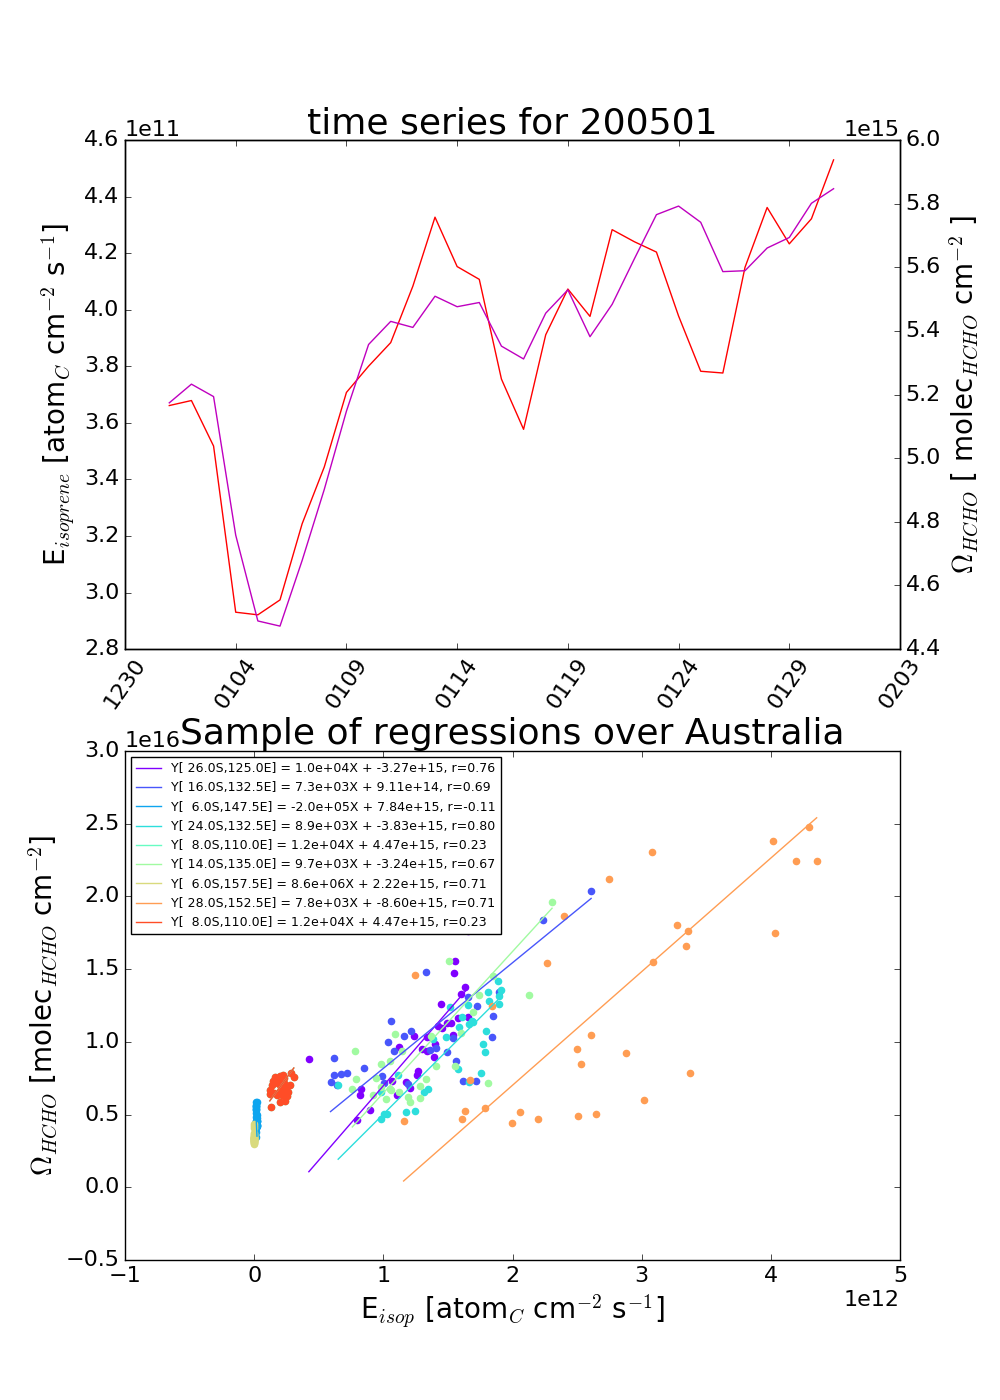
\includegraphics[width=\textwidth]{Figures/Isoprene/E_isop_vs_hcho_series_200501.png}
    %  \caption{%
    %    Top panel: isoprene emissions for January, 2005, shown in red, co-plotted with tropospheric hcho columns, shown in magenta.
    %    Both series are daily averages over Australia.
    %    Bottom panel: (RMA) linear regressions from between emissions of isoprene and tropospheric hcho columns, sampled randomly from the 2$^{\circ}$ by 2.5$^{\circ}$ latitude longitude grid boxes over Australia for the month of January (2005).
    %  }
    %  \label{BioIsop:method:calculation:fig_E_isop_vs_hcho_model_sample}
    %\end{figure}
    
    %% BACKGROUND calculation(s)
    There are two simple ways to determine the modelled background HCHO, one of which involves running the model with no isoprene emissions.%, which shows how much they alter vertical column HCHO.
    Since we have assumed variation in HCHO columns only depends on isoprene emissions, our background term is theoretically identical to this simulated HCHO.
    The other method uses HCHO over the remote Pacific at matching latitudes and times, which emulates how the background is determined for the satellite measured HCHO.
    Figure \ref{BioIsop:method:fig_background_hcho} shows GEOS-Chem total column HCHO with and without isoprene emissions along with amounts over the remote Pacific at the same latitudes.
    The difference in $\Ogc$ over Australia with no isoprene emissions, and $\Ogc$ over the remote pacific (bottom right panel) shows the difference ($\sim 1$ to $3$ \moleccm) between these methods in an example averaged month (January, 2005).
    This difference is relatively small, and may be due to non-isoprene HCHO precursors.
    For consistency with the satellite data, we determine backgrounds using the remote Pacific.
    Background HCHO for any latitude in this thesis is calculated by averaging longitudinally (140\degr W to 160\degr W) the matching latitudes over the remote Pacific.
    %These backgrounds are used when creating the reference sector corrections for satellite measurements (in Section \ref{Model:omiRecalc:RSC}).
    %The background columns are longitudinally averaged from 140\degr W to 160\degr W.
    
    % Figure from chapter_3_isop.py
    \mypic{Figures/OMI_link/GC/GC_background_hcho_200501.png}{%
      Top left: Total column HCHO over Australia using the standard tropchem GEOS-Chem simulation.
      Top right: As top left except over the remote Pacific region at southern mid-latitudes.
      Bottom left: As top left except using the no isoprene emissions GEOS-Chem simulation.
      Bottom right: Difference between the no isoprene emission HCHO columns over Australia, and the remote Pacific HCHO columns from the standard tropchem run at matching latitudes.
      }{\label{BioIsop:method:fig_background_hcho}}
    
    
  \subsection{Calculation of Emissions}
    \label{BioIsop:method:calculation}
   
    Top-down emissions estimates are calculated using OMHCHO (see Section \ref{Model:omhcho}) slant columns and an updated AMF calculated using code by Paul Palmer and Randal Martin, with modifications by Luke Surl (see Section \ref{Model:omiRecalc:ppcode}).
    These emissions are referred to as the a posteriori from here onward, or $\apost$ in formulae.
    
    
    % First: outline of what we do
    % Assumptions already described in outline
    %First I assume that HCHO and isoprene columns are in a steady state, with no horizontal transport, as done in other literature \parencite[e.g.][]{Palmer2003, Millet2006, Bauwens2016}.
    %Another assumption is that isoprene is the only compound enhancing the HCHO levels, which requires that we filter out influence from fires, smoke, and anthropogenic emissions.
    A posteriori emissions are calculated using the linear relationship described in Section \ref{BioIsop:method:slope} using the modelled slope $S$ calculated in the prior section and satellite HCHO columns recalculated in \ref{Model:omiRecalc}:
    \begin{eqnarray} \begin{split}
      \label{BioIsop:method:eqn_Enew}
      \Oomi = & S \times \apost + \Omega_0 \\
      \apost = & \frac{\Oomi - \Omega_{0}}{S}
    \end{split} \end{eqnarray} 
    This is the same as equation \ref{BioIsop:method:slope:eqn_isop_to_hcho}, except now we use the satellite HCHO ($\Oomi$, and $\Omega_0$).
    $\Omega_0$ is calculated using $\Oomi$ in the remote Pacific averaged monthly and longitudinally, for each latitude.
    This leaves $\apost$ as the only unknown once the satellite measurements are processed to match the temporal and horizontal resolution of $S$.
    Figure \ref{BioIsop:method:calculation:fig_E_isop_200501} shows an example of how the a priori compares to the a posteriori, averaged over January, 2005.
    This figure gives a single month of output as an example.
    The a priori exceeds 500\% of the a posteriori in many regions, however this is mostly in regions of low emissions and represents only minor absolute differences. 
    Analysis of the full record is discussed in the results (Section \ref{BioIsop:results}).
    
    
    
    % RENAME TITLES TO a priori and a posteriori
    % RERUN MAKING SURE NEGATIVES ARE REMOVED OR ZEROED
    \begin{figure}
      % Figure from Analyse_E_new.MEGAN_vs_E_new()
      \includegraphics[width=\textwidth]{Figures/OMI_link/Emiss/MEGAN_vs_E_VCC_PP_lr_20050101-20051231.png}
      \caption{%
        Top row: isoprene emissions from GEOS-Chem (a priori, left) simulation and top-down (a posteriori, right) calculations averaged over the month of January, 2005.
        Bottom row: the absolute (left) and relative (right) differences between the two.
      }
      \label{BioIsop:method:calculation:fig_E_isop_200501}
    \end{figure}
    
    
    One potential issue in this top down estimation technique is the low number of valid satellite measurements that may occur due to the higher zenith angles in winter and at higher latitudes.
    When calculating the a posteriori from our modelled slope, negative emissions result wherever measured columns are lower than background amounts (as $\apost = \frac{\Oomi - \Omega_0}{S}$).
    These are set to zero, which increases monthly averages by TODO: $\sim X-Y$~\% ($\sim XX - YY$~atom C cm$^{-2}$ s$^{-1}$) over Australia, with the highest increases occurring during (TODO winter?).
    
  \subsection{Accounting for smearing}
    \label{BioIsop:method:smearing}
    
    In high NO$_x$ ($ > \sim 1 $~ppb) environments, isoprene has a lifetime on the order of 30 minutes, and HCHO can be used to map isoprene emissions with spatial resolution from 10-100~kms \parencite{Palmer2003}.
    In low NO$_x$ conditions, isoprene has a longer lifetime (hours) and may form HCHO further from the source area \parencite{Fan2004,Liu2016a,Liu2017_hpald}.
    Over Australia, NO$_x$ levels are generally low and smearing is therefore expected to be important.
    Smearing limits the horizontal resolution of the linear top-down inversion process, as a finer resolution increases sensitivity to transport.
    %The relatively coarse horizontal resolution (\lowhr) used by GEOS-Chem is advantageous in this aspect.
    Horizontal transport \textit{smears} the HCHO signal so that its source location would need to be calculated using wind speeds and loss rates \parencite{Palmer2001,Palmer2003}.
    Smearing is a measure of how much HCHO in a given grid box was produced from isoprene emitted in a different (upwind) grid box.
    Smearing affects emissions estimates as HCHO enhancements downwind of where precursor emissions occurred lead to misinterpretation of local emissions.
    Smearing affected grid squares are filtered out prior to application of Equation \ref{BioIsop:method:slope:eqn_isop_to_hcho}.
    
    
    %\textcite{Marais2012} additionally use airborn isoprene, MVK $+$ MACR (isoprene oxidation products), and HCHO measurements to check smearing in Africa where there is a sharp gradient of isoprene emitting vegetation from north to south.
    
    \subsubsection{Calculation of smearing}
      \label{BioIsop:method:smearing:calculation}
      
      Smearing has been analysed in several publications \parencite[e.g.][]{Martin2003, Palmer2003, Millet2006, Stavrakou2009, Marais2012, Barkley2013, Zhu2014, Wolfe2016, Surl2018}, and is often calculated using the method used in this thesis, as first described in \textcite{Palmer2003}.
      This involves using two model runs, one of which has isoprene emissions scaled globally by a constant (generally from 0.5 to 2).
      %Another method \parencite[e.g.][]{Stavrakou2009} involves the analysis of an adjoint CTM, however this is computationally expensive and is not pursued here.
      % slope and yields
      %In order to understand the smearing calculation the underlying equations and assumptions must first be understood.
      From Section \ref{BioIsop:method:slope}, Equation \ref{BioIsop:method:slope:eqn_isop_to_hcho} states that the modelled slope ($S$) is the yield of HCHO per C of emitted isoprene divided by HCHO loss rate ($S = \frac{Y_{isop}}{k_{HCHO}}$).
      % smearing defined from two runs of geos chem
      Using two runs of GEOS-Chem with differing isoprene emissions but otherwise identical we have:
      \begin{eqnarray}
        \label{BioIsop:method:smearing:calculation:eqn_runs}
        \begin{split}
        Run_1 :&  \Omega_{HCHO} = S E_{isop} + \Omega_0 \\
        Run_2 :&  \Omega_{HCHO}' = S' E_{isop}' + \Omega_0' 
        \end{split}
      \end{eqnarray}
      There are several assumptions that need to be understood, as these are what is tested by the smearing calculation.
      The initial assumption is that the system is at steady state, with no transport of isoprene affecting HCHO columns, this is the basis for equations \ref{BioIsop:method:smearing:calculation:eqn_runs}.
      It is also assumed that background values ($\Omega_0$) are from oxidation of methane and other long lived VOCs, so that $\Omega_0 = \Omega_0'$.
      Between these two runs we are only changing the $E$ term.
      Chemistry is unchanged so that the yield and loss rate should not change between the two runs: 
      \begin{equation}
        S = S' = \frac{Y_{isop}}{k_{HCHO}}
      \end{equation}
      Equations \ref{BioIsop:method:smearing:calculation:eqn_runs} may then be combined as follows:
      \begin{eqnarray}
        Run_1-Run_2 : \Omega_{HCHO} - \Omega_{HCHO}' = & S E_{isop} - S' E_{isop}' +\Omega_0 - \Omega_0' \notag \\
        \Omega_{HCHO} - \Omega_{HCHO}' = & S \left( E_{isop} - E_{isop}' \right) \notag \\
        \Delta \Omega_{HCHO} = & S \Delta E_{isop}  \notag \\
        \hat{S} \equiv & \frac{\Delta{\Omega_{HCHO}}}{\Delta E_{isop}} \approx \frac{Y_{isop}}{k_{HCHO}} \label{BioIsop:method:smearing:calculation:eqn_hats}
      \end{eqnarray}
      This allows the combination of outputs from the two runs to determine where $\hat{S}$ diverges from expected values for $S$.
      %The modelled slope multiplied by the column HCHO loss rate ($k_{HCHO} = 1/\tau$) should approximate the HCHO yield from isoprene \parencite{Palmer2003, Barkley2013}.
      
      Potential smearing is masked by checking thresholds a daily modelled value for $\hat{S} \approx Y_{isop}/k_{HCHO}$ against thresholds.
      By assuming that midday HCHO lifetime ($\tau = 1/k_{HCHO}$) typically falls within 1.5 to 4~hrs (as seen in the USA \parencite[e.g.][]{Palmer2006,Wolfe2016}) and isoprene to HCHO yield (HCHO per isoprene carbon emitted) lies within the range 0.2 to 0.4 (scenarios estimated in \textcite{Palmer2003}), one can set a simple bound on $\hat{S}$ of $[0.2 \times 1.5, 0.4 \times 4]$~hrs or 1080 to 5760 seconds.
      As NO$_x$ levels across Australia are relatively low, and lower NO$_x$ levels reduce the prompt yield \parencite{Palmer2003,Wolfe2016}, I reduce the threshold range by 20\% and round to the nearest hundred leading for bounding range of 800 to 4600 for $\hat{S}$. 
      This range strikes a balance between unlikely modelled yields and how much data is lost to filtering.
      %Todo?: Show yield and lifetimes from caaba/mecca if possible
      Table \ref{BioIsop:method:smearing:tab_smearing_ranges} compares the smearing filter for Australia used in this thesis to typical slopes used in previous work for other regions.
      %This smearing range captures isoprene to HCHO yields of around 0.16 to 0.32 C per C if HCHO lifetime is assumed to lie within 1.5 to 4 hours.
      %These ranges mean we only use data that is not outside the feasible bounds of yields or lifetimes in Australia.
      
      \begin{table}\begin{threeparttable}
          \caption{Smearing filters or typical slopes ($S$) from literature.}
          \begin{tabular}{ l | c  c  l  >{\centering\arraybackslash}p{3cm} } 
            \toprule
            Publication & min. (s) & max. (s) & type$^a$ & Region \\
            \midrule
            \textcite{Palmer2003}      & 1270 & 2090 & Range & North America$^{b}$ \\
            \textcite{Marais2012}      &      & 4000 & Limits & Africa \\
            \textcite{Barkley2013}$^c$ & 1300 & 1800 & Limits & South America \\
            \textcite{Surl2018}        & 2200 & 4900 & Range & India \\
            In this Thesis             & 800  & 4600 & Limits & Australia \\
            \bottomrule
          \end{tabular}
          \begin{tablenotes} 
            \item a: Slope \textit{range}s are observed or modelled $S$, while smearing \textit{limits} are the applied acceptable limits for $S$. 
            \item b: Slope range for summer only.
            \item c: Assumed HCHO lifetime of 2.5 hours implies yields from 0.14 to 0.2 per C, consistent with box modelling.
          \end{tablenotes}
          \label{BioIsop:method:smearing:tab_smearing_ranges}
        \end{threeparttable}\end{table}
      
      
      To determine which model grid boxes are affected by smearing, we follow \textcite{Marais2012}.
      GEOS-Chem is run with and without isoprene emissions halved, then Equation \ref{BioIsop:method:smearing:calculation:eqn_hats} ( $\hat{S} = \frac{\Delta \Omega_{HCHO}}{\Delta E_{isop}} $) provides $\hat{S}$.
      Here $\Delta$ represents the difference (daily 1300-1400~LT) between default and scaled runs.
      If $\hat{S}$ sits outside the 800-4600 range then we remove that grid square day from both $S$ and subsequent a posteriori calculations.
      A relatively large change in $\Omega_{HCHO}$ compared to local emissions ($\hat{S}>4600$) suggests HCHO production is from non-local isoprene emissions.
      Alternatively, a relatively low value of $\hat{S}$ ($\hat{S}<800$) suggests emissions from the local grid square are being exported before they form HCHO.
      
      
      % Marais 2012 also look at average windspeed and best hcho-isop corelation when hcho is shifted by 0.5 degrees, don't think I can do that with 2.5 degree resolution
      % Marais compare smearing with model estimated yield "
    
    \subsubsection{Sensitivity to smearing}
    
      Smearing can be dependent on local or regional weather patterns, as greater wind speeds will reduce the time any emitted compound stays within the local grid box.
      As such smearing can vary greatly both spatially and temporally.
      Smearing is also sensitive to time of day, season, and latitude, as higher lower insolation results in slower photolysis.
      Figure \ref{BioIsop:method:smearing:fig_smearing_def_2005} shows smearing in summer and winter.
      The smearing filter is more active in winter, especially at higher latitudes.
      The filter removes more data on coastal grid squares as they are more affected by winds and transport.
      Additionally, any grid square with low isoprene emissions will be more sensitive to transport, as the signal is lower.
      During summer data-loss from smearing is only minor (todo: Y\%); however, data-loss peaks in winter (TODO X \%), especially in higher southern latitudes.
      %JENNY NOTE:I don't really understand why you are showing both columns in this figure. I know you did this analysis to figure out how to do smearing, but you are just using the midday emissions in what follows right? Which makes sense anyway because that is when the HCHO obs are from? I would remove the extra column and focus in the text on what this figure says about when, seasonally, smearing is important. Maybe even add autumn and spring here to show the seasonal change.
      
      %Isoprene emissions (E$_{isop}$) are defined in two ways in this figure: left column from daily averaged flux, and right column from and midday (1300-1400~LT) flux. 
      %Essentially the midday isoprene emissions are at the peak of their daily cycle (shown later in Figure \ref{BioIsop:method:scaled:megan_diurnal}) and the effect of smearing is relatively smaller during these hours.
      
      %TODO: UPDATE FIGURE -> Remove old smearing definition, 
      \mypic{/Figures/OMI_link/Filters/smearing_definitions_2005.png}{%
        Seasonally averaged smearing ($\hat{S}$, see text) in summer (DJF) and winter (JJA) from 2005.
        Diamonds represent grid squares which have had at least 1 day removed due to the smearing filter, and red crosses show where more than 45 days ($\sim50\%$) have been removed.
      }{\label{BioIsop:method:smearing:fig_smearing_def_2005}}
      
      
      When limiting smearing ($\hat{S}$) to within 800-4600~s, GEOS-Chem correlations between isoprene emissions and HCHO columns improve marginally and not uniformly (Figure \ref{BioIsop:method:slope:fig_smear_filter_prior}). 
      Where smearing is prevalent, the relationship between a priori emissions and HCHO columns may already be weak due to low actual emissions or unsuitable meteorological conditions.
      Loss of data due to filtering is handled by using multiple years of data for any affected grid square month as follows.
      $S$ and associated regression coefficients ($r$) are calculated monthly.
      If $r<0.4$ then the regression is calculated using multiple years of data for that month.
      This multiple year regression is discarded completely if it also has a coefficient of $r<0.4$, leaving no slope for the grid square for the month.
      %TODO: How often does this happen? where is it most common?
      %potentially where the 95\% confidence interval min and max ratio is too high (too wide).
      %Figure TODO shows GEOS-Chem midday HCHO columns compared against GEOS-Chem emissions of isoprene, over land squares with (red) and without (grey) filtering for smearing.
      
    \subsubsection{Smearing length scale}
    
      
      The expected horizontal transport (prior to reaction) of a precursor can be calculated using the smearing length \parencite{Palmer2003}.
      The distance travelled ($L$) downwind by a precursor ($i$) before forming HCHO can be estimated through:
      \begin{equation*}
        L_{i} = \frac{U}{k_i - k_{HCHO}} \ln{ \left( \frac{k_i}{k_{HCHO}} \right) }
      \end{equation*}
      where $U$ is wind-speed.
      \textcite{Palmer2003} further define a smearing length scale $L_{s,i}$ as the distance downwind where most of the precursor is completely transformed into HCHO.
      Here we use the simplification of $L_{s,isop} \approx \frac{U}{k_{HCHO}}$ as isoprene loss rates (2~h$^{-1}$) exceed those of HCHO (0.25-0.67~h$^{-1}$) by a factor of 3-8.
      These numbers come from assuming HCHO lifetime of 1.5-4~h, and isoprene lifetime of 30~m TODO: cite.
      Throughout most of the year, over most of Australia, monthly averaged wind speeds do not exceed 20~km h$^{-1}$ (\url{http://www.bom.gov.au/jsp/ncc/climate_averages/wind-velocity/} [accessed Feb., 2019]), although daily wind speeds will be highly variable.
      This means that a reasonable upper limit for the smearing length scale is $20 / 0.25 = 80$~km over Australia.
      Grid boxes used in top-down estimation of isoprene emissions describe rectangles with both side lengths approximately 200~km, so generally I do not expect to be overly impacted by smearing.
      %Figure TODO: shows a rough estimate of isoprene smearing length($L_{s,isop}$) in Australia using wind speeds from TODO:, and reaction rates $k_{isop}$, $k_{HCHO}$ from GEOS-Chem.
      %%TODO make this plot!
      The estimated loss rate of HCHO in GEOS-Chem %approximately ranges from 1e6 to 3e6 mol cm$^{-3}$ s${-1}$, 
      is up to three times higher in summer and along the north and eastern regions associated with denser forest regions, when compared against other regions.
      This is largely due to loss rates being proportional to concentrations, and leads to less smearing sensitivity over areas of high isoprene emissions and HCHO concentrations.
       
      %This equation uses the initial VOC column concentration ($[VOC]_0$) at the point of emission and mass balance equations as follows:
      %%TODO: Add intermediate steps
      %\begin{equation}
      %\frac{1}{k_{HCHO}-k_i} \left( k_{HCHO} \exp{ \left[ \frac{-k_i L_{s,i}}{U} \right]} -k_i %\exp{ \left[ \frac{-k_{HCHO} L_{s,i}}{U} \right]} \right) = \frac{1}{e} 
      %\end{equation}
      %with limiting values $L_{s,i} \rightarrow U/k_i$ for $k_i << k_{HCHO}$, and $L_{s,i} \rightarrow U/k_{HCHO}$ for $k_{HCHO} << k_i$.
      
      % Discussion of HCHO and isoprene lifetimes/yields 
      %The half-life of HCHO %to photo-oxidation with hydroxyl radicals 
      %is around 1~hr depending on environmental conditions \parencite{WHO_hcho_guidelines_2010}.
      %This would make the expected lifetime ($\tau = \text{half-life}/\ln{2}$) around 1.4 hours.
      %Over the majority of Australia conditions are relatively clean (low NO$_x$), which extends the expected lifetime.
      
      
      GEOS-Chem daily averaged HCHO lifetime ($\tau$) is calculated using daily averaged surface loss rates ($L_{HCHO}$) and concentrations of HCHO:
      \begin{equation*}
      \tau = \frac{[HCHO]}{L_{HCHO}}
      \end{equation*}
      The expected lifetime of HCHO is determined by assuming loss is linear (first order) and dividing grid box daily averaged concentrations of GEOS-Chem HCHO ($[HCHO]$ in molecules cm$^{-3}$) by their modelled losses ($L_{HCHO}$ in molecules cm$^{-3}$ s$^{-1}$).
      For each grid square over Australia this daily averaged surface lifetime in summer (Jan., Feb.) and winter (Jul., Aug.) is shown in Figure \ref{BioIsop:method:smearing:fig_tau_GC_2005}.
      Additionally lifetimes coloured by location (dots in the top right panel) are shown over time in the bottom panel.
      Note that this figure shows the daily averaged lifetime, as loss rate diagnostics are only available as a daily average.
      Loss rates would maximise at midday (13:00-14:00~LT), along with HCHO concentrations, which makes the estimate shown here an upper limit. 
      This figure highlights the seasonal nature of HCHO lifetime, although midday numbers are expected to have less seasonality than shown here, since midday lifetime will be less affected by how long the daylight lasts.
      % JENNY NOTE: You are writing this in a section about smearing length scale (presumably to determine where you expect smearing to be important, or not). It would therefore be good to tie all this lifetime stuff back to the smearing length scale. You used average k_HCHO above, but what does this actually look like for GEOS-Chem? Would it make sense to show k_HCHO in your plots rather than tau to better equate this to your assumptions? Or even to show the average length scale, assuming a mean wind speed of 20 or 25 kph as you did above?
      Another highlighted issue is the potential latitudinal dependence of HCHO lifetimes, since there is less total insolation leading to lower HCHO loss rates at higher latitudes.
      The overall takeaway is that the accuracy and utility of any top down HCHO precursor estimation technique will be limited by both season and potentially latitude.
      These limitations are due to both data availability (as satellite HCHO uncertainty increases at high zenith angles) and spatial smearing (due to HCHO lifetimes that increase with reduced insolation and temperature).
      
      \mypic{/Figures/OMI_link/Filters/tau_2005.png}{%
        Top left, right: summer (Jan., Feb.) and winter (JJA) averaged daily surface HCHO lifetime ($\tau$). Bottom panel: $\tau$ over the year, coloured by location (see dots in top right panel).
      }{\label{BioIsop:method:smearing:fig_tau_GC_2005}}
      
    %Nitrous oxide is N2O. You are after nitric oxide (NO) or nitrogen oxides (NO2)
    \subsubsection{NO$_x$ dependence}
      
      %There is an important non-linear relationship between VOCs, HO$_x$, and NO$_x$. 
      NO$_x$ concentration directly affects the fate of VOCs in the atmosphere, influencing HCHO production by isoprene.
      In low NO$_x$ environments, reported HCHO yields from isoprene are around 0.2 - 0.3 C per C (or 100-150 molar \%), while in high NO$_x$ environments this value becomes two to three times higher \parencite{Palmer2003, Wolfe2016}.
      %\textcite{Wolfe2016} also see background HCHO doubling in high NO$_x$ regions.
      %\textcite{Wolfe2016} determine that going from NO$_X = 0.1$ to $2.0$ ppbv triples the prompt yield of HCHO, from 0.3 to 0.9 ppbv ppbv$^{-1}$ due to isoprene, while the background HCHO doubles.
      Some values for HCHO yield from prior literature are shown in Table \ref{BioIsop:method:tab_VOCLiteratureYields}.
      %Increasing NO$_x$ from 0.1~ppbv to 2.0~ppbv can triple the prompt isoprene yield of HCHO,  %from 0.3 to 0.9 ppbv ppbv$^{-1}$
      %and double background HCHO \parencite{Wolfe2016}.
      
      %Conversions between HCHO per unit C yield and molar \% yield from species X are given by the equation $ Y_{molar \%} = 100 \times C_X \times Y_{HCHO \,C^{-1}}$, where $C_X$ is how many carbon are within species X (5 for isoprene).
      %For instance a 200\% molar yield of HCHO from isoprene implies 1 mole of C$_5$H$_8$ becomes 2 mole HCHO which is a 0.4 HCHO per unit C yield.
      %      
      % yields from Atkinsen2003
      %isoprene
      %0.63 0.10 Tuazon and Atkinson (1990a)
      %0.57 0.06 Miyoshi et al. (1994)
      % a-pinene
      %0.23 0.09 Noziere et al. (1999a)
      %0.19 0.05 Orlando et al. (2000)
      % b-pinene
      %0.54 0.05 Hatakeyama et al. (1991)
      %0.45 0.08 Orlando et al. (2000)
      
      % molar HCHO yield per unit carbon equal to HCHO molar percent yield(per carbon)? or some conversion?
      \begin{table} \begin{threeparttable}
          \caption{ Isoprene to HCHO yields and lifetime.}% against oxidation by OH. }
          \begin{tabular}{  l  l  l  l  }
            \toprule
            HCHO Yield    & Lifetime     & NO$_x$ background & Source   \\
            (molar \% )   &              &                   &          \\
            \midrule 
            315$\pm$50      &            & High          & a        \\ 
            285$\pm$30      &            & High          & a        \\ 
            225             & 35 min     & High          & b        \\ % Done
            150             &            & Low           & b        \\ % Done
            150             &            & Low           & d        \\
            450             &            & High          & d        \\
            235             &            & 1~ppbv        & e        \\
            150             &            & 0.1~ppbv      & e        \\
            %          $\alpha$-Pinene & 28$\pm$3        &        & Low                & c        \\ 
            %          & X$\pm$3         &        & X                  & d        \\ 
            %          & 230$\pm$90      &        & High        & a        \\ 
            %          & 190$\pm$50      &        & High        & a        \\ 
            %          & 19              & 1 hour &              & b        \\ % Done
            %          & 210             &        & 1~ppbv        & e        \\
            %          & 70              &        & 0.1~ppbv      & e        \\
            %          $\beta$-Pinene  & 65$\pm$6        &        & Low           & c      \\ 
            %          & X$\pm$3         &        & X             & d      \\ 
            %          & 540$\pm$50      &        & High          & a     \\ 
            %          & 450$\pm$80      &        & High          & a      \\ 
            %          & 45              & 40 min &              & b      \\ % Done
            %          Methane 	      & 100             & 1 year  &             & b     \\ 
            %          Ethane          & 180             & 10 days &             & b     \\ 
            %          Propane         & 60              & 2 days  &             & b     \\ 
            %          Methylbutanol   & .13(per C)    & 1 hour  &             & b     \\ 
            %          HCHO            & 100             & 2 hour  &             & b     \\ 
            %          Acetone         & .67(per C)      & 10 days &             & b     \\ 
            %          Methanol        & 100             & 2 days  &             & b     \\ %Done
            \bottomrule
          \end{tabular}
          \begin{tablenotes} % \item makes new lines
            \item a \textcite{AtkinsonArey2003}: Table 2, Yield from Isoprene reaction with OH, two values are from two referenced papers therein.
            \item b \textcite{Palmer2003}: lifetimes assume [OH] is 1e15 mol cm$^{-3}$.
            \item c \parencite{Lee2006}: Calculated through change in concentration of parent and product linear least squares regression.
            Estimates assume 20$^\circ$~C conditions.
            \item d \textcite{Wolfe2016}: ``prompt yield'': change in HCHO per change in isop$_0$.
            $[isop]_0=[isop]\exp(k_1[\mathrm{OH}]t)$; where $k_1$ is first order loss rate.
            Effectively relates HCHO abundance with isoprene emission strength.
            \item e \textcite{Dufour2009}: One-day yields from oxidation modelled by CHIMERE, using MCM reference scheme.
            %\item f Calculated using PTR-MS and iWAS on SENEX campaign data.
          \end{tablenotes}
          \label{BioIsop:method:tab_VOCLiteratureYields}
        \end{threeparttable} \end{table}
      
      %% NO$_2$ from the OMNO2d product provides daily mid-day measurements that we compare to output from GEOS-Chem NO$_2$ (see Section \ref{Model:GC:NOx}).
      %\textcite{Travis2016} show how NO$_x$ can be used to examine model bias in ozone (potentially due to NO$_2$ bias) over the USA.
      The effect of NO$_2$ on smearing can be seen in Figure \ref{BiogIsop:Method:smearing:fig_smearing_vs_nox}.
      This plot shows how smearing over Australia compares to satellite NO$_2$, with smearing distributions binned by NO$_2$ both with and without filtering for smearing.
      At lower NO$_2$ levels the smearing is often 2-4 orders of magnitude above the upper threshold. 
      This abruptly decreases at around $5 \times 10^{14} $~molec cm$^{-2}$ NO$_2$.
      There is also a higher number of data points below the lower threshold before that same NO$_2$ level, showing that transport is a bigger issue at NO$_2 < 5 \times 10^{14} $~molec cm$^{-2}$. 
      %This is an issue in Australia since NO$_2$ levels sit at roughly this threshold.
      Due to the coarse resolution of the model, many regions with low NO$_2$ also have low isoprene emission levels, and this filtering does not remove too many data points from biogenic-dominated regions.
      
      %% FIGURE SHOWS SMEARING BINNED BY NOX
      % Figure made in test_filters.smearing_nox() 
      \mypic{Figures/OMI_link/Filters/smearing_nox_200501.png}{%
        Top left: OMNO2d tropospheric NO$_2$ columns (NO$_2$: molec cm$^{-2}$) averaged into \lowhr horizontal bins for Jan, 2005.
        Right: Scatter plot of NO$_2$ against smearing calculations from GEOS-Chem ($\hat{S}$), with points above and below the smearing threshold range of 900-5200~s coloured red and blue respectively. 
        Points are binned by NO$_2$ with and without the smearing filter applied (orange and magenta respectively).
        Overplotted is the mean and standard deviation (error bars) within each bin. 
        Due to the logarithmic Y scale we only show the positive direction of standard deviations for unfiltered data.
        Bottom left: Daily NO$_2$ scattered against smearing with (magenta) and without (orange) applying the smearing filter. This plot is a zoomed out version of the right panel.
      }{\label{BiogIsop:Method:smearing:fig_smearing_vs_nox}}
      
  \subsection{Running GEOS-Chem using a posteriori emissions}
  \label{BioIsop:method:scaled}
    
    After creating our a posteriori isoprene emissions estimate, we run GEOS-Chem again with biogenic emissions scaled to match the new estimate. 
    This is performed by applying a seasonal scaling factor $\alpha$, based on the multi-year monthly average difference between midday a priori and a posteriori emissions at \lowhr horizontal resolution.
    $\alpha$ is the ratio between the multi-year averaged monthly emissions from GEOS-Chem $\apri$ and the a posteriori $\apost$: 
    \begin{equation} \label{BioIsop:method:scaled:eqn_alpha}
        \alpha = \frac{\apost}{\apri}
    \end{equation}
    This seasonal scaling retains shorter time-scale variability and meteorological dependencies, while ensuring the multi-year monthly averaged emissions match.
    %Short time-scale variability is largely due to meteorological parameters such as temperature and light, etc..
    Initially $\alpha$ is uniformly set to 1 globally.
    Where top down emissions exist and $\apri$ is non-zero, we can set $\alpha$ using Equation \ref{BioIsop:method:scaled:eqn_alpha}.
    $\alpha$ is applied through the emissions module in GEOS-Chem where isoprene emissions are calculated.
    First all the new midday (13:00-14:00~LT) emissions (per grid box) are combined forming a multi-year monthly mean, which can be compared to the a priori equivalent.
    Missing values for $\alpha$ when $\apri$ are zero are a negligible issue since the dominant discrepancies between estimates occurs during summer when high emission rates are overestimated.
    Figure \ref{BioIsop:method:scaled:fig_alpha_mya_series} shows $\alpha$ for the average January and June over 2005-2012, along with a time series of $\apri$ and $\apost$ and $\alpha$ calculated for Sydney, and their multi-year seasonal average.
    
    % Figure from TODO:???
    % UPDATE TO a priori and a posteriori - remove 'examine' from second row
    \mypic{Figures/OMI_link/new_emiss/alpha_mya.png}{%
      Row 1: $\alpha$ for the average January (left) and June (right) over 2005-2012.
      Row 2: $\apri$ (magenta, left axis), $\apost$ (cyan, left axis), and  $\alpha$(black, right axis) multi-year monthly averages calculated for Sydney.
      Row 3: Monthly averages of the same terms in Row 2.}{\label{BioIsop:method:scaled:fig_alpha_mya_series}}
    
    Top-down emission rates calculated in this work are in units of atom C cm$^{-2}$ s$^{-1}$.
    In order to calculate the emissions in kg, each grid square is multiplied by its area, and then daily emissions are assumed to follow a sine wave peaking at the midday value.
    Figure \ref{BioIsop:method:calculation:fig_daily_emissions_kg} shows how the daily approximation of total emitted isoprene per grid square is calculated.
    Daytime hours are estimated per month, from 14~hrs (Jan) to 10~hr (Jul) (\url{https://en.wikipedia.org/wiki/Daytime}).
    This approximation is required since OMI observations occur at midday, when isoprene emissions are at their diurnal peak.
    
    %TODO % can picture sit on one side of page? or can I squish caption? 
    \mypicw{0.5\textwidth}{Figures/Emissions_per_day.png}{%
      Total daily isoprene emissions (in kg) is represented by the area under the sine wave.
    }{\label{BioIsop:method:calculation:fig_daily_emissions_kg}}
    
% UP TO HERE JENNY
\section{Results}
  \label{BioIsop:results}
  
  Australia is roughly $7.7 \times 10^6$ km$^{2}$, with heterogeneous environmental conditions.
  The results presented in this section are frequently split into five regions that are differentiated by colour, as shown in Figure \ref{BioIsop:results:fig_subregions}.
  
  % figure from Analysis_E_isop.py.show_subregions()
  \mypic{Figures/OMI_link/subregions.png}{%
    Sub-regions used in subsequent figures.
    Australia-wide averages will be black or grey, while averages from within the coloured rectangles will match the colour shown here.
  }{\label{BioIsop:results:fig_subregions}}
  

  \subsection{Updated emissions}
    \label{BioIsop:results:emissions}
    
    Figure \ref{BioIsop:results:emissions:fig_time_series_vs_megan} shows a priori emissions over Australia and the updated emissions calculated using OMI.
    The figure shows the time series (daily midday averages) their absolute differences (a priori - a posteriori) over 2005.
    The seasonal cycle and the difference between the two metrics is clear, with much higher spring and summer averages in the a priori.
    The northern region also shows a departure from the Australian mean in the a priori data from mid March through to November, which is not seen in the a posteriori.
    This overestimate by the a priori may be caused by overly high emission factors pushed up by high temperatures during the dry season.
    January and February also show a low feature in the a posteriori data, which may be due to filtering (TODO check data count), or may have been caused by meteorological factors (TODO Check if drought or fires occurred).
    This figure is repeated using monthly means (of the daily midday estimates) in Figure \ref{BioIsop:results:emissions:fig_time_series_vs_megan_monthly} over 8 years from 2005 to 2012.
    Over the entirety of Australia the seasonal cycle of emissions is shown to be overestimated by the a priori.
    The difference between a priori and a posteriori estimates differs between regions, and some noise can be seen in the monthly time series due to data loss (TODO: check data counts).
    While most regions generally adhere to this behaviour of overestimation, the northern region of Australia follows a different cycle of bias.
    Northern Australia appears to be overestimated throughout the year, however occasional low points occur in summer in which the a priori is near to or lower than the a posteriori.
    One potential reason is the onset of the wet season (November-April) that disrupts the ecosystems and limits satellite measurement through increased cloud coverage.
    
    % TODO: Update to remove 'Days since yyyymmdd labels
    % Figure from Analyse_E_isop.py -> E_regional_time_series()
    \mypic{Figures/OMI_link/Emiss/E_zones_PP_lr.png}{%
      Biogenic emissions of isoprene from GEOS-Chem (running MEGAN), which is our a priori in column 1, and the emissions calculated using the OMI top down inversion, which is our a posteriori in column 2.
      %Row 1: overall averaged daily midday emission rates, from 1, Jan, 2005 to 1, May, 2013.
      Row 1: time series of daily midday averages for all of Australia along with several subregions (shown in row 1). 
      The black lines and grey areas show the Australian mean and inter-quartile range respectively, while the coloured lines show the mean within subregions as shown in Figure \ref{BioIsop:results:fig_subregions}.
      The overall regional averages are shown at the end of the time series by horizontal lines.
      Row 2: Absolute differences: a priori - a posteriori.
      TODO: remove spines along top and middle of top row
    }{\label{BioIsop:results:emissions:fig_time_series_vs_megan}}
    
    % also Analyse_E_isop.E_regional_time_series()
    \mypic{Figures/OMI_link/Emiss/E_zones_PP_monthly_lr.png}{ %
      As Figure \ref{BioIsop:results:emissions:fig_time_series_vs_megan} using monthly medians of the daily midday emissions estimates.
    }{\label{BioIsop:results:emissions:fig_time_series_vs_megan_monthly}}
    
    
    TODO Figure shows the satellite data counts over time and summer vs winter maps from the OMHCHORP dataset, along with uncertainty in each region 
    
    
    Figure \ref{BioIsop:results:emissions:fig_megan_vs_Enew_regional_mya} shows the multi-year monthly mean and IQR of daily midday isoprene emissions estimates, averaged regionally. 
    Months outside of May to August show the a posteriori lower than the a priori, except in the south eastern region.
    Here the difference is only prominent during February, TODO check if this may be because of data point counts.
    %JENNY NOTE:
    TODO: Which regions show best correlation? Worst? Why might that be, and what does it mean?
    
    % Figure from Analyse_E_isop.py -> E_regional_multiyear()
    % TODO update titles and add Y axis, update legend
    % TODO run over 2005-2012
    \mypic{Figures/OMI_link/Emiss/E_zones_multiyear_PP_lr.png}{ %
      The multi-year monthly mean (lines) and IQR (shaded) of midday (13:00-14-00~LT) isoprene emissions estimates. 
      %Estimates come from MEGAN run by GEOS-Chem (E$_{GC}$), and the OMI top-down technique (E$_{OMI}$).
      A priori emissions are shown by the dashed lines and hatched shaded areas show the IQR.
      A posteriori emissions are shown using the solid lines, with IQR shown by unhatched shaded areas.
      Colours denote the region over which the monthly average was taken, as in Figure \ref{BioIsop:results:fig_subregions}.
    }{\label{BioIsop:results:emissions:fig_megan_vs_Enew_regional_mya}}
    
    Figures \ref{BioIsop:results:emissions:fig_daily_egressions} and \ref{BioIsop:results:emissions:fig_monthly_egressions} show how the distributions of a posteriori emissions compare to the a priori in each region during summer months (DJF) with zeros removed from both distributions. % zeros or negatives in top-down estimate are from hcho lower than background
    Figure \ref{BioIsop:results:emissions:fig_daily_egressions} shows the daily midday distributions, binned hexagonally and coloured to show data-point frequency.
    There is only weak correlation between daily estimations, and the distributions are quite different with more variance shown by the a priori.
    This is likely due to the filtering applied to both satellite data (e.g. whenever cloud coverage exceeds 40\%) and a posteriori emission calculations.
    Figure \ref{BioIsop:results:emissions:fig_monthly_egressions} displays the regressions between monthly averages of the same data. 
    In the monthly averages a stronger correlation is apparent, with regression coefficients ranging from 0.48 to 0.78 across regions.
    The portion of this correlation due to seasonality is examined by re-running the regression after subtracting the multi-year monthly average from each dataset.
    TODO: run regression after removing seasonal average and see how r and slope are affected.
    
    \mypic{Figures/OMI_link/Emiss/daily_Egressions.png}{%
      Scatter plot (binned hexagonally to show data-point frequency) along with the distributions of MEGAN (y axis) and the top down estimate (x axis).
      This figure is based on summer (DJF) midday values over multiple years.
      Coloured by regions shown in Figure \ref{BioIsop:results:fig_subregions}.
    }{\label{BioIsop:results:emissions:fig_daily_egressions}}
    
    % UPDATE: fix Y axis labels -> a priori, X axis -> a posteriori, add units, remove negative axes, REMOVE legend point marker
    % Figure from Analyse_E_isop.distributions_comparison_regional()
    \mypic{Figures/OMI_link/Emiss/monthly_Egressions.png}{%
      Scatter plot of a priori emissions against a posteriori using monthly averaged grid squares as regression datapoints.
      Data points are created using monthly averages (of midday emissions) for each grid box for each month of summer (DJF) within each region shown.
      Multiple years of data are used, meaning if a region has 10 grid boxes, the 8 years of data will add up to $10 \times 3 \times 8 = 240$ data points minus filtered and zero emission squares.
      Plots are coloured by regions matching those shown in Figure \ref{BioIsop:results:fig_subregions}.
      The linear best fit regression is inset into each plot along with the line equation and regression coefficient.
    }{\label{BioIsop:results:emissions:fig_monthly_egressions}}
    
    
  \subsection{A posteriori GEOS-Chem output}
  \label{BioIsop:results:new_emiss}
    
    This section examines how outputs from GEOS-Chem change after applying a scaling factor $\alpha$ (see Section \ref{BioIsop:method:scaled}) to biogenic isoprene emissions.
    Here we need to be careful of notation, outputs from the scaled GEOS-Chem run will be denoted by a superscript $\alpha$.
    For example column HCHO from GEOS-Chem before and after scaling are $\Ogc$ and $\Ogca$ respectively.
    %unscaled GEOS-Chem biogenic emissions are the a priori, top down midday emissions are the a posteriori, and emissions from the scaled GEOS-Chem run are denoted E$^{\alpha}_{GC}$.
    
    Figure \ref{BioIsop:method:scaled:megan_diurnal} shows the multi-year monthly mean daily cycle of isoprene emissions from GEOS-Chem, along with the top-down midday estimate, for an example grid box located 2.5\degr West of Sydney.
    TODO: Analysis of this and lead into more analysis of differences
    
    % TODO: add suptitle: diurnal isoprene emissions 
    \mypic{Figures/OMI_link/Emiss/MEGAN_monthly_daycycle.png}{ %
      The diurnal cycle of MEGAN emissions averaged by month over 1, Jan, 2005 to TODO, 2013 are shown with lines, while top-down emissions estimates are shown with plus symbols.
      MEGAN emissions are estimated hourly per \lowhr horizontal grid box, shown here are the area averages (denoted by colour, see Figure \ref{BioIsop:results:fig_subregions}).
      Top-down estimates are similarly grouped by colour, and shown at the 13:00~LT mark for each month.
      }{\label{BioIsop:method:scaled:megan_diurnal}}
    
    \subsubsection{HCHO levels}
  
      After running GEOS-Chem with isoprene emission scaled to match the a posteriori, we first check $\Ogc$ and $\Ogca$ outputs against $\Oomi$ over January in 2005 in Figure \ref{BioIsop:results:emissions:fig_prelim_new_emiss_HCHO}.
      In every region $\Ogca$ is closer to the satellite measured amounts with biases lowering from 50-120\% down to 30-50\%.
      Multiple years are combined to form a similar plot showing the same metrics seasonally in Figure TODO.
      
      % TODO: update to use scaled run and tropchem run in legend as Ogc and Ogca
      % figure from initial version of tests/test_new_emissions.hcho_ozone_series
      \mypic{Figures/OMI_link/new_emiss/HCHO_total_columns_20050101_20050131.png}{%
        Daily mean total column HCHO amounts from GEOS-Chem with (new emissions run) and without (tropchem run) a posteriori scaled isoprene emissions, along with the original OMI HCHO columns.
        Each row shows the average over regions in Figure \ref{BioIsop:results:fig_subregions}. }{\label{BioIsop:results:emissions:fig_prelim_new_emiss_HCHO}}
      
    
      %As is done in \textcite{Emmerson2016}, 
      We also examine the effects of scaling isoprene emissions on the correlation between modelled and satellite based HCHO columns.
      Figure TODO: shows the regressions between GEOS-Chem tropospheric column amounts of HCHO and satellite columns for two runs of GEOS-Chem: a) using standard MEGAN emissions, b) using our updated emissions.
      The a posteriori emissions interpolated over the day are lower than a priori GEOS-Chem emissions by X\% per year (from XX to YY \tgpyr) over Australia.
      GEOS-Chem HCHO at midday is reduced by X\% when isoprene emissions are scaled to down.
      % didn't end up boosting monoterpenes... , although if we boost monoterpenes by X\% where the isoprene emissions were lowered then 
      
      Wollongong FTIR measurements (see Section \ref{Model:datasets:wollongong_ftir}) provide vertical profiles of HCHO that can be converted to total column amounts using modelled air densities.
      This is the only non-satellite long-term record of vertical profile HCHO available in Australia and we use it here to examine trends and seasonality.
      The time series for HCHO is shown in figure TODO, along with GEOS-Chem output before and after updating isoprene emissions.
      TODO: discuss plot here
      
      TODO: Figure showing campaign data against model and recalculated model.
      
      
      Figure TODO shows how Wollongong FTIR HCHO profiles compare against GEOS-Chem modelled HCHO before and after isoprene scaling is performed. 
      The regressions show improvement/no improvement TODO 
      
      Figure todo shows how the longer term FTIR HCHO measurements compare against modelled HCHO before and after changing isoprene emissions
  
    \subsubsection{Ozone levels}
  
      Isoprene breaks down in the atmosphere and can lead to increased ozone concentrations, especially when mixing with polluted urban air masses which contain high NO$_X$ concentrations.
      Figure \ref{Conclusions:ozone:fig_new_emiss_series_O3} shows surface level (up to $\sim 150$~m altitude) ozone concentrations over 2005 before and after scaling modelled isoprene emissions.
      Reducing isoprene emissions lowers surface ozone concentrations by TODO: XX to YY \% in summer, and XX to YY \% in winter.
      The direct correlation between reduced emissions and surface ozone (Figure TODO) shows that reduced emissions directly relate to reduced ozone concentrations, and using multiple years enhances/reduces the relationship.
      A look at the regression using only summer data reveals a stronger/weaker relationship, analyse per region (TODO).
      
      TODO Figure showing isoprene vs ozone time series and correlation.
      
      The relatively clean atmosphere over the majority of Australia is likely to be NO$_x$ limited outside of major population centres.
      This means that cities may have higher sensitivity to changes in modelled isoprene emissions than shown here, since we are examining large area averages which are mostly non-urban.
      TODO: Notes about ozone exposure from State of the Environment report 2016.
      
      
      TODO: Figure shows modelled surface ozone concentrations and their differences between model runs over an average summer (DJF). 
      Figure TODO shows the same over an average winter (JJA).
      Figure TODO compares the summer differences to surface NO emissions (modelled), and total column NO (satellite).
      
    
    \subsubsection{Trends}
    \label{BioIsop:results:new_emiss:trends}
    
      %Plot time series of isoprene emissions for each region pre and post change
      % subtract seasonal mya cycle and show trend and p value for trend being non-zero.
      Figure \ref{BioIsop:results:new_emiss:trends:fig_emission_anomalies} shows monthly deseasonalised a priori and a posteriori midday emission anomalies for each region.
      First the emissions are spatially averaged within each region to form a daily time series of midday emission rates, this is averaged into monthly data, and then the multiyear monthly mean is subtracted to form the anomaly series.
      Any anomaly which is greater than 3 standard deviations from the mean is removed (these points can be seen as crosses in Figure \ref{BioIsop:results:new_emiss:trends:fig_emission_anomalies}).
      An ordinary least squares linear regression is then performed to look for any significant trend.
      A trend is considered significant if the p-value from a Wald test is less than 0.05.
      The midday emissions show no significant trends over the 8 year period from 2005-2012.
      The same process is repeated for surface ozone, surface HCHO, and surface NO$_2$, with anomaly series shown in Figures \ref{BioIsop:results:new_emiss:trends:fig_ozone_anomalies} to \ref{BioIsop:results:new_emiss:trends:fig_no2_anomalies}.
      None of these metrics shows any significant changes in trend due to scaling isoprene emissions.
      Some trends are no longer significant in surface HCHO, however none of the trends change sign.
      
      % trend figures from chapter_3_isop.trend_analysis()
      \mypic{Figures/OMI_link/new_emiss/trend_isop.png}{%
        A priori (row 1) and a posteriori (row 2) emissions anomaly from multiyear monthly mean, split by region (see Figure \ref{BioIsop:results:fig_subregions}).
        }{\label{BioIsop:results:new_emiss:trends:fig_emission_anomalies}}
      
      
      \mypic{Figures/OMI_link/new_emiss/trend_O3.png}{%
        A priori (row 1) and a posteriori (row 2) surface ozone anomaly from multiyear monthly mean, split by region (see Figure \ref{BioIsop:results:fig_subregions}).
      }{\label{BioIsop:results:new_emiss:trends:fig_ozone_anomalies}}
      
      \mypic{Figures/OMI_link/new_emiss/trend_hcho.png}{%
        A priori (row 1) and a posteriori (row 2) surface HCHO anomaly from multiyear monthly mean, split by region (see Figure \ref{BioIsop:results:fig_subregions}).
      }{\label{BioIsop:results:new_emiss:trends:fig_hcho_anomalies}}
      
      \mypic{Figures/OMI_link/new_emiss/trend_NO2.png}{%
        A priori (row 1) and a posteriori (row 2) surface NO$_2$ anomaly from multiyear monthly mean, split by region (see Figure \ref{BioIsop:results:fig_subregions}).
      }{\label{BioIsop:results:new_emiss:trends:fig_no2_anomalies}}
      
      
      %Table \ref{BioIsop:results:new_emiss:trends:tab_trend_slopes} shows monthly slopes for ozone, HCHO, and NO$_2$ before and after scaling isoprene emissions, where the regression is significant (Wald test $p$ value $< 0.05$).
      %In summary there are/are not trends seen over the 2005-2012 period before and or after scaling isoprene emissions.
      
      
  %    area:key,   new_emiss,   tropchem
  %    isop monthly anomaly
  %    region, [ slope, regression coeff, p value for slope non zero]
  %    Aus &  [ m=-3.65e-03,  r=-0.472, p=0.000 ]   & \
  %    significant!  isop Aus
  %    SE &  [ m=-1.32e-02,  r=-0.397, p=0.000 ]   & \
  %    significant!  isop SE
  %    NE &  [ m=-1.09e-02,  r=-0.386, p=0.000 ]   & \
  %    significant!  isop NE
  %    Mid &  [ m=-5.69e-03,  r=-0.389, p=0.000 ]   & \
  %    significant!  isop Mid
  %    SW &  [ m=-6.48e-04,  r=-0.048, p=0.643 ]   & \
  %    N &  [ m=-5.18e-03,  r=-0.247, p=0.015 ]   & \
  %    significant!  isop N
  %    isop monthly anomaly (scaled)
  %    region, [ slope, regression coeff, p value for slope non zero]
  %    Aus &  [ m=-1.33e-03,  r=-0.433, p=0.000 ]   & \
  %    significant!  isop Aus
  %    SE &  [ m=-6.01e-03,  r=-0.431, p=0.000 ]   & \
  %    significant!  isop SE
  %    NE &  [ m=-3.45e-03,  r=-0.385, p=0.000 ]   & \
  %    significant!  isop NE
  %    Mid &  [ m=-1.79e-03,  r=-0.384, p=0.000 ]   & \
  %    significant!  isop Mid
  %    SW &  [ m=-4.78e-04,  r=-0.120, p=0.248 ]   & \
  %    N &  [ m=-1.98e-03,  r=-0.184, p=0.074 ]   & \
  %    SAVED  Figs/new_emiss/trend_isop.png
  %    area:key,   new_emiss,   tropchem
  %    hcho monthly anomaly
  %    region, [ slope, regression coeff, p value for slope non zero]
  %    Aus &  [ m=-4.91e-04,  r=-0.275, p=0.007 ]   & \
  %    significant!  hcho Aus
  %    SE &  [ m=-2.36e-03,  r=-0.351, p=0.000 ]   & \
  %    significant!  hcho SE
  %    NE &  [ m=-1.55e-03,  r=-0.305, p=0.003 ]   & \
  %    significant!  hcho NE
  %    Mid &  [ m=-9.54e-04,  r=-0.233, p=0.022 ]   & \
  %    significant!  hcho Mid
  %    SW &  [ m=-4.49e-05,  r=-0.012, p=0.906 ]   & \
  %    N &  [ m=-6.92e-04,  r=-0.119, p=0.247 ]   & \
  %    hcho monthly anomaly (scaled)
  %    region, [ slope, regression coeff, p value for slope non zero]
  %    Aus &  [ m=-1.99e-04,  r=-0.179, p=0.080 ]   & \
  %    SE &  [ m=-1.65e-03,  r=-0.397, p=0.000 ]   & \
  %    significant!  hcho SE
  %    NE &  [ m=-6.50e-04,  r=-0.238, p=0.021 ]   & \
  %    significant!  hcho NE
  %    Mid &  [ m=-2.34e-04,  r=-0.110, p=0.286 ]   & \
  %    SW &  [ m=1.22e-05,  r=0.006, p=0.953 ]   & \
  %    N &  [ m=-2.14e-04,  r=-0.057, p=0.584 ]   & \
  %    SAVED  Figs/new_emiss/trend_hcho.png
  %    area:key,   new_emiss,   tropchem
  %    NO2 monthly anomaly
  %    region, [ slope, regression coeff, p value for slope non zero]
  %    Aus &  [ m=-2.86e-05,  r=-0.106, p=0.307 ]   & \
  %    SE &  [ m=-2.73e-04,  r=-0.320, p=0.002 ]   & \
  %    significant!  NO2 SE
  %    NE &  [ m=-1.19e-04,  r=-0.226, p=0.027 ]   & \
  %    significant!  NO2 NE
  %    Mid &  [ m=-7.87e-05,  r=-0.176, p=0.089 ]   & \
  %    SW &  [ m=1.54e-05,  r=0.035, p=0.739 ]   & \
  %    N &  [ m=1.31e-04,  r=0.170, p=0.102 ]   & \
  %    NO2 monthly anomaly (scaled)
  %    region, [ slope, regression coeff, p value for slope non zero]
  %    Aus &  [ m=-2.48e-05,  r=-0.100, p=0.336 ]   & \
  %    SE &  [ m=-2.54e-04,  r=-0.315, p=0.002 ]   & \
  %    significant!  NO2 SE
  %    NE &  [ m=-1.03e-04,  r=-0.215, p=0.035 ]   & \
  %    significant!  NO2 NE
  %    Mid &  [ m=-5.17e-05,  r=-0.135, p=0.196 ]   & \
  %    SW &  [ m=-1.62e-05,  r=-0.038, p=0.716 ]   & \
  %    N &  [ m=1.01e-04,  r=0.151, p=0.149 ]   & \
  %    SAVED  Figs/new_emiss/trend_NO2.png
  %    area:key,   new_emiss,   tropchem
  %    O3 monthly anomaly
  %    region, [ slope, regression coeff, p value for slope non zero]
  %    Aus &  [ m=4.40e-03,  r=0.073, p=0.480 ]   & \
  %    SE &  [ m=-2.80e-02,  r=-0.287, p=0.005 ]   & \
  %    significant!  O3 SE
  %    NE &  [ m=-6.54e-03,  r=-0.073, p=0.480 ]   & \
  %    Mid &  [ m=-4.04e-03,  r=-0.041, p=0.693 ]   & \
  %    SW &  [ m=1.28e-02,  r=0.204, p=0.047 ]   & \
  %    significant!  O3 SW
  %    N &  [ m=1.47e-02,  r=0.102, p=0.326 ]   & \
  %    O3 monthly anomaly (scaled)
  %    region, [ slope, regression coeff, p value for slope non zero]
  %    Aus &  [ m=6.11e-03,  r=0.111, p=0.280 ]   & \
  %    SE &  [ m=-2.33e-02,  r=-0.268, p=0.009 ]   & \
  %    significant!  O3 SE
  %    NE &  [ m=-4.08e-03,  r=-0.050, p=0.632 ]   & \
  %    Mid &  [ m=-3.47e-03,  r=-0.042, p=0.686 ]   & \
  %    SW &  [ m=1.42e-02,  r=0.259, p=0.011 ]   & \
  %    significant!  O3 SW
  %    N &  [ m=1.41e-02,  r=0.106, p=0.306 ]   & \
  %    
      
  %    % From Chapter_Isop.trend_analysis
  %    % a priori and a posteriori showed no significant trends
  %    \begin{table}\begin{threeparttable}
  %      \caption{Regional deseasonalised monthly anomaly trends}
  %      \begin{tabular}{ l  c  c  c } 
  %        \toprule
  %        region & ozone & HCHO & NO$_2$ \\
  %        \midrule
  %        \textbf{a priori emissions}$^a$ & & & \\
  %        Aus & m & m & m \\ 
  %        \midrule
  %        \textbf{a posteriori emissions}$^b$ & & & \\
  %        Aus & m & m & m \\ 
  %        \bottomrule
  %      \end{tabular}
  %      \begin{tablenotes} 
  %        \item a: GEOS-Chem output using default isoprene emissions
  %        \item b: GEOS-Chem output using scaled isoprene emissions
  %      \end{tablenotes}
  %      \label{BioIsop:results:new_emiss:trends:tab_trend_slopes}
  %    \end{threeparttable}\end{table}
      
      
  \subsection{Literature comparisons}
    
    % 
    When comparing GEOS-Chem (which runs MEGAN) emissions to those calculated using our top-down inversion, we see a decrease of around 29\tgpyr ($66\%)$.
    \textcite{Sindelarova2014} see a 41\tgpyr decrease in Australia when introducing soil moisture parameterisation.
    Global and Australian emissions estimates for isoprene still range widely due to the emission models sensitivities to inexact parameters including leaf area indices, plant functional type emission factors, and meteorological factors.
    Table \ref{BioIsop:results:emissions:tab_emissions_Tg} shows yearly isoprene emissions from this work and some other works for Australia.
    Our a posteriori estimate of 19 \tgpyr suggests isoprene emissions may be lower than any bottom up estimates, and is close to the top-down estimate performed in \textcite{Bauwens2016} of 26 \tgpyr.
    Figure \ref{BioIsop:results:emissions:fig_tga_comparison_map} shows how this decrease is distributed spatially, with $\apri$ and $\apost$ in \tgpyr calculated as a multi-year mean.
    Across all of Australia we see large reductions of total emissions using the new top-down estimate.
    
    \mypic{Figures/OMI_link/Emiss/tga_map.png}{%
      Top row: multi-year mean emissions in \tgpyr from $\apri$ (GEOS-Chem; running MEGAN) and $\apost$ (top-down emissions) respectively.
      $\apost$ uses an assumed sinusoidal daily cycle, with daylight hours perscribed for each month: see Section \ref{BioIsop:method:calculation}).
      Bottom left and right shows the absolute and relative differences respectively.}{\label{BioIsop:results:emissions:fig_tga_comparison_map}}
    
    
    %TODO: Update with 2005-2013 rather than just 2005-2007
    %global MEGAN: 471.518577725
    %aus MEGAN: 45.4326831613
    %aus OMI  : 16.4731027389
    
    \begin{table}\begin{threeparttable}
      \caption{Isoprene emissions (Tg/yr)}
      \begin{tabular}{ l  c  >{\arraybackslash}p{10cm} } 
        \toprule
        Australia & notes \\
        \midrule
        43(2) & a) GEOS-Chem: 2005-2010 \\ % 445(18) globally
        19(2) & b) Top-down: 2005-2010 \\
        $\sim 80$ & c) \textcite{Sindelarova2014}: 1980-2010 \\ % 590 globally
        26-94 & d) \textcite{Bauwens2016}: 2005-2013\\
        %&  535 & \textcite{Guenther2012}: \\
        
        %26-94 & 272-570 & c) \textcite{Bauwens2016}: 2005-2013\\
        \bottomrule
      \end{tabular}
      \begin{tablenotes} 
        \item a: MEGAN diagnostics based on 3-hourly averages
        \item b: Based on daily peak emissions integrated over a sinusoidal daily curve
        \item c: MEGAN run using MERRA meteorology.  
        \item d: Range shown here based on 3 different models and one top-down inversion
      \end{tablenotes}
      \label{BioIsop:results:emissions:tab_emissions_Tg}
    \end{threeparttable}\end{table}
  
  
  \subsection{Comparison with available measurements}
    \label{BioIsop:results:measurements}
    TODO: % TODO: campaign analysis compared to GEOS-Chem
    Analyse comparison of grid box with campaigns of measurements
    
    Comparison between ground-based measurements and large (\lowhr) averaged grid squares suffers from representation error.
    Figure \ref{BioIsop:results:measurements:fig_gridbox} shows the SPS and MUMBA measurement sites, along with an outline of the \lowhr model grid box.
    The grid box is the area over which GEOS-Chem outputs are averaged, a rectangle with edge lengths of roughly 200~km$^{2}$.
    The urban footprint of Sydney and Wollongong can be seen, along with some ocean, forest, and rural regions, which will all affect the model output and other calculations averaged here.
    Due to high uncertainty in components of the top-down emissions estimate, temporal resolution is also limited.
    MUMBA, SPS1 and SPS2 each provide relatively few data points, which are compared against surface level concentrations from GEOS-Chem before and after scaling the biogenic emissions.
    %campaigns measured isoprene concentrations while our estimate is of emissions.
    
    %figure from Jenny
    \mypic{Figures/gridmapsmall_sites.png}{% 
      grid box at \lowhr containing SPS, and MUMBA campaign data.}{\label{BioIsop:results:measurements:fig_gridbox}}
    
    Figure \ref{Model:datasets:SPS:fig_GC_comparison} shows GEOS-Chem output in the grid square containing Sydney overlaid on SPS measurement data.
    Superficially the comparison is not too bad between these two datasets.
    %, however GEOS-Chem output is the daily average over \lowhr (latitude by longitude).
    This figure shows at a glance how the measurements compare to modelled data, and also the limited nature of the temporal and spatial scale of available measurements.
    TODO: if possible use midday isoprene multi-year averages, and error bars? then update discussion.
    The SPS data is point-source and taken during the daytime when isoprene is higher, so it is very likely that GEOS-Chem HCHO and isoprene output is in fact too high since the daily average should not match the peak of the measurements.
    
    % TODO Update with comparison before and after scaling isoprene emissions
    \mypic{Figures/OMI_link/GC_vs_Campaigns_20050131-20050601.png}{%
      Comparison between GEOS-Chem HCHO concentrations in the grid square containing Sydney for the duration of the SPS 1 and 2 campaigns}{\label{Model:datasets:SPS:fig_GC_comparison}}
    
    % Figure showing apriori and apostiori for any locatation can be made by test_E_new.location_timeseries()
    
    
    Figure TODO shows how isoprene compares against measurements from the MUMBA and SPS campaigns (described in Section \ref{Model:datasets}) both before and after scaling isoprene emissions to match the top-down estimation.
    TODO: discuss results and differences, does isoprene improve?
    
    
    MUMBA data captured concentrations at the surface in Wollongong, and is compared in figure TODO against simulated HCHO concentrations in the first level ($\sim$0 - 150~metres) over corresponding dates.
    GEOS-Chem midday concentrations are shown, along with Wollongong bottom-level FTIR measurements to compare against the MUMBA data.
    TODO Discussion of comparison.
    
  \subsection{HCHO Products and yield}
    \label{BioIsop:results:HCHOYield}
    
    Isoprene reaction chains are diverse, with many branches forming HCHO. 
    HCHO production yields are often classed into two categories: first generation HCHO yield and total (or molar) yield.
    First generation yield refers to the amount of HCHO produced per unit isoprene consumed by initial oxidation.
    Total yield refers to time dependent yield of HCHO over multiple oxidation stages \parencite{Wolfe2016}.
    %\textcite{Wolfe2016} define prompt yield as the change in formaldehyde per unit change in initial isoprene emissions.
    %$[ISOP]_0=[ISOP]\exp(k_1[\mathrm{OH}]t)$; where $k_1$ is first order loss rate.
    In this work yield ($Y_{isop}$) is not calculated as the slope ($S = Y_{isop}/k_{HCHO}$) can be used instead.
    This section shows a brief analysis of HCHO lifetimes ($\tau$) at midday.
    
    By assuming yield $Y_{isop}$ lies between 0.2 and 0.4, we find a range for midday lifetimes of HCHO using equation \ref{BioIsop:method:slope:eqn_isop_to_hcho}:
    \begin{eqnarray*}
      S = & \frac{Y_{isop}}{k_{HCHO}} \\
      \tau \equiv & \frac{1}{k_{HCHO}} \\
      \tau = & \frac{S}{Y_{isop}}
    \end{eqnarray*}
    $\tau$ is heavily influenced by assumed yield, and improved methods of estimating yield over Australia are required to improve this estimate.
    Figure \ref{BioIsop:results:HCHOYield:fig_Lifetime}: shows the GEOS-Chem HCHO lifetime estimated throughout the year.
    There is a clear seasonal cycle with longer lifetimes in winter months.
    A clear June (and sometimes March, July and August) increase in HCHO lifetimes is shown, which is caused by the reduced winter HCHO concentrations, temperature, and insolation.
    These factors may limit the utility of any top-down emissions estimation technique using HCHO in the winter months.
    The figure is produced using filtered slope information from 2005, and outliers along with low data availability in some months is an issue.
    Noise in the southwest and middle regions may be indicative of heavy filtering, potentially driven by westerly winds which can bring transported polution and also lead to smearing.
    
    % Plot/calculation from GC_tests.yield_and_lifetime()
    \mypic{Figures/OMI_link/GC/HCHO_lifetime.png}{ %
      Monthly area averaged HCHO lifetime ($\tau$ in hours), with IQR shaded.
      Solid lines show lifetime assuming yield is 0.2, and 0.4 (higher and lower lines respectively).
      Coloured by regions shown in Figure \ref{BioIsop:results:fig_subregions}.
    }{\label{BioIsop:results:HCHOYield:fig_Lifetime}}
    
    
\section{Uncertainty}
\label{BioIsop:uncertainty}
  
%  \subsection{Summary}
%    \label{BioIsop:uncertainty:summary}
  Uncertainties introduced through the inversion process are difficult to adequately quantify. 
  We can identify the uncertainties in the linear regression used to relate HCHO to isoprene emissions, as well as in the satellite data product, however these uncertainties lack verification against measurements.
  Even as this top-down inversion attempts to remedy the lack of measurement over Australia, it suffers from the lack of data-points against which it can be verified.
  
  This section identifies and quantifies the overall uncertainties of calculating isoprene emissions using OMHCHO and GEOS-Chem in the top-down method.
  The major source of uncertainty lies in TODO, which is due to TODO.
  Uncertainty in satellite HCHO is seasonally dependent, with better signal during the summer. 
  Good OMI measurements are less frequent at high solar zenith angles, which depends on latitude as well as season, which exacerbates the winter uncertainty.
  %This limits temporal resolution of isoprene emissions estimates.
  Table \ref{BioIsop:uncertainty:tab_uncertainties} shows the estimated uncertainty calculated in this work in summer and winter over each region described by Figure \ref{BioIsop:results:fig_subregions}.
  How each of these terms is calculated is laid out in the following subsections.
  
  \begin{table}\begin{threeparttable}
      \caption{Uncertainty estimations.}
      \begin{tabular}{ l | c  c  c | c c c} 
        \toprule
        Region & $\Delta \apost$ & $\Delta \Oomi$ & $\Delta S$ 
          & $\Delta \apost$ & $\Delta \Oomi$ & $\Delta S$ \\
         & Summer & & & Winter & & \\
        \midrule
          Aus & & & & & & \\
          SE & & & & & & \\
          NE & & & & & & \\
          ... & & & & & & \\
        \bottomrule
      \end{tabular}
      %\begin{tablenotes} 
        %\item a: 
      %\end{tablenotes}
      \label{BioIsop:uncertainty:tab_uncertainties}
    \end{threeparttable}\end{table}
    
    
  
  \subsection{Top down emissions}
    \label{BioIsop:uncertainty:eomi}
    
    Important factors in the calculation of isoprene emissions using OMI HCHO include the modelled a priori, the relationship between HCHO and isoprene, and satellite measurements.
    Uncertainty in each of these terms is quantified before being combined in quadrature to give the uncertainty estimate of the a posteriori.
    Additional biases may arise due to the filters applied to satellite data and model output, and where possible these are assessed. 
    
    %filtering techniques for pyrogenic and anthropogenic influences, and the regression model for determining the isoprene to HCHO yield.
    The final determination of top-down emissions comes from equation \ref{BioIsop:method:eqn_Enew}: 
    \begin{equation*}
      \apost=\frac{\Oomi - \Omega_{OMI,0}}{S}
    \end{equation*}
    Assuming each term is independent, we use the following quadrature rules to estimate random error in $\apost$:
    \begin{align}
      \mathtt{z=x+y:} \, \Delta{z} & = \sqrt{(\Delta{x})^2 + (\Delta{y})^2} \\
      \mathtt{z=x/y:} \, \Delta{z} & = z \sqrt{(\frac{\Delta{x}}{x})^2 + (\frac{\Delta{y}}{y})^2} \label{BioIsop:uncertainty:eqn_quadrature_divide} 
    \end{align}
    Which leads to the uncertainty estimation for our a posteriori emissions as follows
    \begin{align}
      \Phi & \equiv \Oomi - \Omega_{OMI,0}   \notag \\
      \Delta{\Phi} & = \sqrt{(\Delta{\Oomi})^2 + (\Delta{\Omega_{OMI,0}})^2}  \label{BioIsop:uncertainty:eomi:eqn_delta_Phi} \\
      \Delta{\apost} &= \apost \times \sqrt{(\frac{\Delta{\Phi}}{\Phi})^2 + (\frac{\Delta{S}}{S})^2} \label{BioIsop:uncertainty:eomi:eqn_delta_apost}
    \end{align}
    
    To quantify $\Delta{\apost}$ we determine the uncertainty in underlying terms: $\Delta{S}$, $\Delta{\Oomi}$, and $\Delta{\Omega_{OMI,0}}$. 
    For $\Delta{S}$ ($\Ogc = S \times \apri + \Omega_{OMI,0}$ from equation \ref{BioIsop:method:slope:eqn_isop_to_hcho}) we examine related GEOS-Chem output in Section \ref{BioIsop:uncertainty:Model}, since $S$ comes directly from the monthly linear regression of modelled isoprene emissions and column HCHO.
    Uncertainty in terms $\Oomi$, and $\Omega_{OMI,0}$ come from both the OMHCHO slant columns ($SC$) and the $AMF$ calculated to transform them into vertical columns ($\Omega = \frac{SC}{AMF}$ from equation \ref{Model:AMF:eqn_AMFFrac}).
    Section \ref{BioIsop:uncertainty:satellite} describes these calculations.
    
    
    Figure TODO shows the average summer and winter random uncertainty over Australia, along with a time series of total emissions and the error bars using monthly averaged data and MEGAN emissions for reference.
    TODO brief analysis of spatial uncertainty stuff
    
    
  
  \subsection{Model Uncertainty}
    \label{BioIsop:uncertainty:Model}
    
    $\apost$ depends partly on the product it is trying to improve, as modelled yield is based on MEGAN run by GEOS-Chem.
    The uncertainty in the RMA regression slope between model HCHO and emissions ($\Oomi$ and $\apri$ respectively) is used to estimate the $\Delta S$ within Equation \ref{BioIsop:uncertainty:eomi:eqn_delta_apost}.
    This is a simple method of approximating the uncertainty of this term, only accounting for monthly uncertainty of the slope calculation.
    It does not take into account uncertainty in the underlying model, nor uncertainties arising from temporal or spatial resolution issues.
    Figure TODO shows the multi-year mean summer and winter $\Delta S$ over Australia.
    Analysis todo
    For comparison \textcite{Palmer2006} found $\frac{\Delta S}{S}$ to be 30\%, after comparison with another chemical model and in situ measurements.
    
    To improve understanding of uncertainty in S would require further analysis of GEOS-Chem yield and sensitivities over Australia, ideally along side representative measurements.
    Here we present a brief analysis of how GEOS-Chem HCHO and isoprene concentrations and variances compare to in situ measurements from MUMBA, SPS1, and SPS2.
    Comparison caveats are that in situ point measurements are quite different to modelled (large) area averages, and that these measurements only take place in one grid box within Australia.
    We see model bias of TODO: difference for isoprene conc before and after, HCHO conc before and after, in the $\sim 4$ months of available measurements.
    Figure TODO shows the measured and modelled metrics for the comparable times.
    
    
    % Filtering
    Filtering for spatial smearing (see Section \ref{BioIsop:method:smearing}) reduces the number of data points making up our regression slope $S$. 
    The process generally improves the linear relationship, and where it does not a multi-year average (or in the worst cases no value at all) is used in lieu of monthly $S$ data.
    The thresholds for the smearing filter are based on literature based overseas, a better approximation of HCHO lifetimes and yields as well as properly accounting for seasonality and regional NO$_x$ concentrations would improve the filter.
    The filtering process is accounted for in the calculation of $\Delta S$, and the overall effect on uncertainty is limited, so we do not analyse it further.
    
    
    % Biases
    Model biases are not analysed in this thesis, except to note that they would impact both preliminary OMI calculations as well as affecting the modelled slope. 
    %Yield calculations are performed at low resolution (2\degr x 2.5\degr) which may lead to overestimation \parencite{Yu2016}.
    
    %Isoprene to HCHO yield between low and high NO$_x$ (0.1 to 1~ppbv respectively) conditions has been estimated through box modelling to be 1.9 to 2.4 mol mol$^{-1}$ in \textcite{Bauwens2016}.
    
  % Subsection?
  \subsection{Satellite Uncertainty}
    \label{BioIsop:uncertainty:satellite}
    
    
    % Summary of satellite error
    There are three main sources of error in the satellite HCHO columns:
    \begin{enumerate}
      \item Fitting error from the OMI retrieval.
      \item Uncertainty in AMF calculations.
      \item Uncertainty of HCHO background.
    \end{enumerate}
    Fitting error is provided by the OMI product and reduced through spatial and temporal averaging.
    %We found taking the eight day gridded average with horizontal resolution of \highhr (latitude by longitude) typically reduces uncertainty by a factor of 1.5 to 4.
    AMF uncertainty can be determined through comparison of GEOS-Chem output to measured HCHO columns.
    Here we use 30\% as a rough estimate of error in this term, since measurements over Australia are lacking.
    %validated against the total column of HCHO at Wollongong using FTIR measurements from the (TODO: Nicholas Jones roof HCHO citation here).
    Since we expect oceanic background HCHO to be invariant, variance in remote ocean HCHO can be used as a rough estimate of background uncertainty.
    % How it's calculated here
    Uncertainty in satellite HCHO ($\Delta{\Omega}$) from literature and calculated here is listed in Table \ref{BioIsop:uncertainty:eomi:tab_lit_uncertainties}.
    %TODO: background uncertainty
    For simplicity, uncertainty in the HCHO background is assumed to be negligible compared to the AMF in this work.
    Further simplification is made by assuming that the relative error of vertical columns is not altered by the process of applying a reference sector correction (see Section \ref{Model:omiRecalc:RSC}).
    
    Provided with the OMI product is the measurement of uncertainty in each pixel, calculated by SAO from the backscattered solar radiation fit \parencite{Abad2015,Abad2016}.
    Uncertainty introduced through AMF calculation needs to be additionally determined to give a representation of the confidence in vertical column amounts.
    We use the uncertainty in each pixel averaged over our \lowhr grid squares for each day and divided by the square root of the number of pixels.
    This is considered to be the error in the slant column ($\Delta SC$), which is combined with our assumed relative AMF error ($\frac{\Delta AMF}{AMF}$) of 30\% .
    $\Delta \Oomi$ and $\Delta \Omega_{OMI,0}$ are calculated for Equation \ref{BioIsop:uncertainty:eomi:eqn_delta_apost} through applying the quadrature rule from Equation \ref{BioIsop:uncertainty:eqn_quadrature_divide} as follows:
    \begin{align}
    \Omega  & = \frac{SC}{AMF} \notag \\
    \Delta \Omega & = \Omega \sqrt{ ( \frac{\Delta SC}{SC} )^2 + ( 0.3 )^2 } 
    \end{align}
    Figure TODO shows the multi-year monthly average of the satellite uncertainty for each sub-region and all of Australia.
    TODO analysis.
    
    %\textcite{Millet2006, Palmer2006} both examine OMI HCHO columns over North America and determine overall uncertainty to be 40\%, with most of this coming from cloud interference.
    \begin{table}\begin{threeparttable}
      \caption{Uncertainties in literature and here.}
      \begin{tabular}{ c  c  l } 
        \toprule
        uncertainty & location & notes \\
        \midrule
        40\% & North America & (a) mostly due to cloud interference \\
        26\% & North America & (b) with cloud fraction less than 20\% \\
        30-40\% & global & (c) GOME-2 instrument \\
        $>60\%$ & Mid-latitude & (c) GOME-2 instrument in winters \\
        X\% & Australia & accumulated uncertainty in calculation \\
        X\% & Australia & range found when scaling satellite HCHO \\
        \bottomrule
      \end{tabular}
      \begin{tablenotes} 
        \item a: \textcite{Millet2006,Palmer2006}
        \item b: \textcite{Millet2008}
        \item c: \textcite{DeSmedt2008,DeSmedt2012}
      \end{tablenotes}
      \label{BioIsop:uncertainty:eomi:tab_lit_uncertainties}
    \end{threeparttable}\end{table}
    
    % How others calculated it
    \textcite{Palmer2006} calculate the error in AMF through combining estimates of error in the UV albedo database ($\sim 8$\%), model error based on in situ measurements, cloud error  ($20-30$\%) \parencite{Martin2003}, and aerosol errors ($<20$\%), totalling AMF error of around $\sim 30$\% (calculated in quadrature).
    TODO: calculate this uncertainty.
    Compare this error estimate with that of \textcite{Curci2010}, where the error in b) and c) are respectively found to be 30\% and 15\% based on their analysis of CHIMERE.
    \textcite{Millet2008} also examine this uncertainty and determine an overall uncertainty ($1\sigma$) of $25-27\%$ in HCHO vertical columns with calculated AMFs where cloud fraction $< 0.2$.
    % another way to calculate delta Oomi
    One method of finding overall satellite uncertainty involves using the variance over the remote Pacific (15\degr S to 15\degr N, and 180\degr W to 120\degr W) \parencite[][]{DeSmedt2012,DeSmedt2015}.
    % abbreviation? BIRA use another method, and calculate the standard deviation of HCHO over the remote Pacific ocean as the uncertainty \parencite{DeSmedt2012, DeSmedt2015}.
    In the remote Pacific, it can be assumed that HCHO variations are weak, with concentrations remaining steady in the short term ($\sim 1$ month).
    This means the standard deviation over this region can be used as a proxy for determination of the instrument error.
    \textcite{DeSmedt2012} found satellite HCHO uncertainty to be $30-40\%$ for the GOME-2 instrument by combining slant column systematic and random errors.
    For mid latitude winters they saw an excess of 60\% uncertainty.
    % maybe TODO: calculate this also and compare with explicit calculations from second paragraph
    
    % Bias
    In order to calculate the bias or systematic error, an understanding of biases in the underlying terms is required, since there is little in the way of comparable measurements.
    % satellite biases:
    OMHCHO has been seen to underestimate HCHO by up to 40\%, although this amount is regionally dependent \parencite{Zhu2016,DeSmedt2015,Barkley2013}).
    Satellite HCHO may also suffer from $\sim13\%$ overestimation when taking a monthly average due to only measuring on relatively cloud-free days \parencite{Surl2018}.
    Since our a posteriori is linearly related to the satellite HCHO, any bias is directly transferred.
    We note therefor that our product may be biased by up to 40\% due to satellite bias.
    This may be complicated further if the satellite bias over Australia does not match the bias over the remote Pacific at corresponding latitudes.
    However we can not quantify bias over Australia due to insufficient measurements.
    % Model biases
    GEOS-Chem biases would affect the recalculation of HCHO, but they are assumed to be minimal in this thesis.
    %model HCHO overestimation due to coarse resolution (over prediction of low-NO$_x$ oxidation pathway \parencite{Yu2016}.
    Since we lack sufficient suitable measurements to estimate satellite bias over Australia, we assume bounds on potential satellite biases based on literature of up to 40\%.
    
    
    \subsubsection{Sensitivity to vertical column recalculation}
      \label{BioIsop:uncertainty:satellite:AMF}
      OMI HCHO vertical columns are recalculated using GEOS-Chem V10.01 a priori HCHO and air density profiles (see Chapter \ref{Model}).
      The recalculation is assumed to be no more or less uncertain than that used to calculate the product provided AMF.
      The pixel SC uncertainty from the OMHCHO product is not changed by recalculating the AMF, and is used as is, as shown in Section \ref{BioIsop:uncertainty:satellite}.
      Here we examine the sensitivity of the isoprene emissions estimation technique to the AMF recalculation method.
      Through looking at how the emissions change based on whether we use the AMF provided (AMF$_{OMI}$), the AMF with shape factor recalculated but the default scattering weights (AMF$_{GC}$), or the fully recalculated AMF (AMF$_{PP}$).
      
      Figure todo shows the emissions over Australia averaged within January 2005.
      TODO: analysis of differences
      
      
      TODO: Figure goes here:... 
      A priori emissions and a posteriori estimates using satellite pixels recalculated using the different AMFs.
      Row 1: calculation using corrected vertical columns that implement the original OMI AMF.
      Row 2: as row 1, updating shape factors to use GEOS-Chem output.
      Row 3: as rows 1 and 2, using the code from Paul Palmer's group to completely recalculate the AMF.
      
      
      Figure todo shows emissions over time from a single grid square, estimated by MEGAN (black) and the three top-down estimates, using \lowhr horizontal resolution.
  
    \subsubsection{Sensitivity to filtering}
    \label{BioIsop:uncertainty:satellite:fire_filter}
    
    %Look at emissions estimates with and without the fire filter applied
    Figure TODO shows emissions estimates for January 2005 with and without filtering for anthropogenic and pyrogenic influences
    TODO: update plot and Analysis
    
%    \mypic{Figures/OMI_link/Emiss/FireFilter200501.png}
%    {Top left shows the a posteriori emissions, while the top right shows same calculations without applying any fire or smoke filter.
%     Bottom left shows the absolute difference between them, while bottom right shows the relative difference.}
% {\label{BioIsop:uncertainty:Fire:fig_emiss_without_fire_filter}}
    
    % TODO: Emissions Averages and differences over the year with and without a fire filter 
    
    
\section{Conclusions and implications}
  \label{BioIsop:conclusions}
  TODO: Brief summary of results and implications...
  
  Our top down biogenic isoprene emission estimate shows that MEGAN overestimates emissions in summer by up to a factor of 5.
  The overestimation is spatially and temporally diverse and leads to model overestimation of HCHO.
  By applying a monthly gridded scaling factor based on the multi-year monthly difference model emissions and our top down a posteriori, HCHO bias can be improved from 50-120\% down to 30-50\% (TODO: update that number for summer season rather than the 2005 January it is based on).
  
  Model overestimation of biogenic isoprene emissions also lowers simulated surface ozone concentrations by several percent.
  This improves our understanding of biogenic emissions impact on surface ozone levels, and could improve certainty in simulated ozone exceedances.
  
  What else?



% Extras for potential paper output 
%  
%  \authorcontribution{}
%  \competinginterests{The authors declare that they have no conflict of interest.}%
%  \textit{Data availability.} All GEOS-Chem model output is available from the authors upon request.
%  %\disclaimer{disclaimer}
%  \begin{acknowledgements}
%    This research is supported by an Australian Government Research Training Program (RTP) Scholarship.
%  \end{acknowledgements}
  